%%%% for public version, toggle \draftfalse in setup2modes.tex
%    (that removes all comments, the blog)

% reducesymm/cgang/2modes.tex    this is master file:    pdflatex 2modes
%     then:    pdflatex def2modes; bibtex def2modes; pdflatex def2modes; pdflatex def2modes

% until 2012-08-20 this was in svn repo siminos/cgang/2modes.tex

\documentclass[aip,cha,
reprint,
secnumarabic,
nofootinbib, tightenlines,
nobibnotes, showkeys, showpacs,
superscriptaddress,
%preprint,%
%author-year,%
%author-numerical,%
]{revtex4-1}

\newcommand{\version}{2modes ver. 2.3, Nov 11 2014}
% Predrag                   ver. 2.3, Nov 11 2014
% Predrag                   ver. 2.2, Jul 24 2014
% Predrag                   ver. 2.1, Jul 14 2014
% Burak                     ver. 2.0, Jul  8 2014
% Predrag                   ver. 1.3, May 11 2014
% Burak                     ver. 1.2, May  6 2014
% Predrag                   ver. 1.1, Nov 16 2013
% Burak                     ver. 1.0, Oct  6 2013
% Predrag                   ver. 0.3, Aug  1 2012
% Predrag                   ver. 0.2, Apr 30 2012}
% Predrag from atlas12      ver. 0.1, Apr 25 2012}

        \input setup2modes
        \input def2modes

\begin{document}

\title[Periodic orbit analysis of a system with continuous symmetry]
{Periodic orbit analysis of a system with continuous symmetry - a tutorial}

\author{Nazmi Burak Budanur}
\email{budanur3@gatech.edu}
\affiliation{
 School of Physics and Center for Nonlinear Science,
 Georgia Institute of Technology,
 Atlanta GA 30332
}
\author{Daniel Borrero-Echeverry}
\affiliation{
 School of Physics and Center for Nonlinear Science,
 Georgia Institute of Technology,
 Atlanta, GA 30332
}
\affiliation{
 Department of Physics,
 Reed College,
 Portland OR 97202
}
\author{Predrag Cvitanovi\'{c}}
\affiliation{
 School of Physics and Center for Nonlinear Science,
 Georgia Institute of Technology,
 Atlanta GA 30332
}
    \ifdraft
\date{\today}
    \else
\date{14 November 2014}
   \fi

\begin{abstract}
Dynamical systems with translational or rotational symmetry arise
frequently in studies of spatially extended physical systems, such as
Navier-Stokes flows on periodic domains. In these cases, it is natural to
express a state of the fluid in terms of a Fourier series truncated to a
finite number of modes. Here we study a 4-dimensional two-mode
SO(2)-equivariant model of this type, the smallest possible truncation
that retains the symmetry while remaining high-dimensional enough to
allow for chaotic dynamics. A crucial step in analysis of such a system
is symmetry reduction. We use the model to illustrate different
symmetry-reduction schemes. Its relative equilibria are conveniently
determined by rewriting the dynamics in terms of a symmetry-invariant
polynomial basis. However, for study of chaotic dynamics, the `method of
slices', applicable also to very high-dimensional problems, is
preferable. We show that a Poincar\'e section within the `slice' can be
used to further reduce this flow to what is for all practical purposes a
unimodal map. This enables us to systematically determine all relative
periodic orbits and their symbolic dynamics up to any desired period. We
then compute several dynamical averages using relative periodic orbits
and discuss the convergence of such computations.
\end{abstract}

\pacs{02.20.-a, 05.45.-a, 05.45.Jn, 47.27.ed, 47.52.+j, 83.60.Wc}
\keywords{
symmetry reduction,
equivariant dynamics,
relative equilibria,
relative periodic orbits,
periodic orbit theory,
slices,
moving frames, chaos
}
\maketitle

\begin{quotation}
Periodic orbit theory provides a way to compute dynamical averages for
chaotic flows by means of {\cycForm s} that relate the time averages of
observables to the spectra of unstable periodic orbits. Standard
{\cycForm s} are valid under the assumption that the stability
multipliers of all periodic orbits have a single marginal direction
corresponding to time evolution, and are hyperbolic in all other
directions. However, if a dynamical system has $N$ continuous symmetries,
periodic orbits are replaced by relative periodic orbits, invariant
$(N+1)$-dimensional tori with marginal stability in $(N+1)$ directions.
These exact invariant solutions arise in studies of turbulent flows, such
as the pipe flow or the plane Couette flow, where the translational
symmetries of the flow are approximated by carrying out simulations in
periodic domains. A state of the fluid can then be expressed as a Fourier
series, truncated to a large but finite (from tens to thousands) set of
Fourier modes. This paper is a tutorial on how such problems are to be
analyzed using periodic orbit theory. We illustrate all steps of
\rpo s analysis on what is arguably the simplest such dynamical system, a
`\twomode' model.
\end{quotation}

\section{Introduction}
\label{s:intro}

Recent experimental observations of travelling waves in pipe flows have
confirmed dynamical systems theory intuition that the invariant solutions
of \NSe\ play an important role in shaping the \statesp\ of turbulent
flows\rf{science04}. When one recasts fluid flow equations in a
particular basis, the outcome is an infinite dimensional dynamical system
that is often equivariant under transformations such as
translations, reflections and rotations. For example, when a periodic
boundary condition is imposed along the streamwise direction, equations
for pipe flow retain their form under streamwise translations, azimuthal
rotations and reflections about the central axis, \ie, they are invariant
under the actions of $\SOn{2} \times \On{2}$. In that case it is natural
that the states of the fluid be expressed in a Fourier basis. However,
as the system evolves the nonlinear terms in the equations mix the
Fourier modes, and thus the state of the system evolves both along
symmetry directions and directions transverse to them.
This phenomenon in dynamical systems with continuous symmetries
complicates their \statesp, and gives rise to the high dimensional coherent
solutions such as \reqva\ and \rpo s, which take on the roles played by
\eqva\ and \po s in flows without symmetry.

This paper is a tutorial that works through an example in order to
illustrate step-by-step how periodic orbit theory is applied to flows
with continuous symmetries, an analysis that should ultimately be applied
to turbulent flows, once sufficiently many exact invariant solutions
become numerically accessible. For this purpose, we study a \twomode\
\SOn{2} equivariant flow, of minimal dimensionality required for chaotic
dynamics. The paper is organized as follows: In \refsect{s:symm} we
define basic concepts and briefly review the relevant symmetry reduction
literature. In \refsect{s:twoMode}, we introduce the \twomode\ model
system, describe several of its representations, and utilize a
symmetry-reduced polynomial representation to find the only \reqv\ of the
system. In \refsect{s:numerics}, we show how the \mslices\ can be used to
quotient the symmetry and reduce the dynamics onto a symmetry-reduced
\statesp, or `\slice'. A Poincar\'e section within the \slice\ then
reduces the 4\dmn\ chaotic dynamics in the full \statesp\ to a
1-dimensional unimodal Poincar\'e return map. This return map is then
used to construct a finite grammar symbolic dynamics for the flow, and
determine {\em all} \rpo s up to a given period. In \refsect{s:DynAvers},
these orbits are used as input to various {\cycForm s} in order to calculate
dynamically interesting observables. In \refsect{s:concl},
we discuss possible applications of the \mslices\ to various spatially
extended systems. \refAppe{s:newton} describes the multi-shooting method used 
to calculate the \rpo s. \refAppe{s:schur} discusses how periodic Schur 
decomposition can be used to determine their Floquet multipliers, which can 
easily differ by 100s of orders of magnitude even in a model as simple as the 
\twomode\ system.

\section{Continuous symmetries}
\label{s:symm}

A dynamical system $\dot{\ssp}=\vel(\ssp)$ is said to be \emph{equivariant} 
or \emph{\Group-equivariant} under the symmetry group \Group\ transformations 
if
\beq
	\vel( \ssp )
    =  \matrixRep(\LieEl)^{-1}\vel(\matrixRep(\LieEl)\ssp)
	\,
\ee{equiv}
for every \statesp\ point $\ssp \in \pS$ and every element $\LieEl \in
\Group$, where \LieEl\ is an abstract group element, and 
$\matrixRep(\LieEl)$ is its $[d\!\times\!d]$ matrix representation.
Infinitesimally, the equivariance condition \refeq{equiv} is expressed as
a vanishing Lie derivative\rf{DasBuch}
\beq
  \Lg \, \vel(\ssp)  - \Mvar(\ssp) \, \groupTan(\ssp) =0
  \,,
\ee{inftmInv}
where
$\Mvar(\ssp)$ is the $[d\!\times\!d]$ \stabmat\, with elements
$\Mvar_{ij}(\ssp)={\pde \vel_i}/{\pde\ssp_j}|_{\ssp}$, $ \groupTan(\ssp)
= \Lg \ssp $ is the group tangent at $\ssp$, and $\Lg$ is the
$[d\!\times\!d]$ generator of infinitesimal transformations, such that
$\matrixRep(\theta) = \exp(\theta\Lg)$, with phase $\theta \in [0,2\pi)$
parametrizing the group action. (We shall interchangeably use notations
$\matrixRep(\LieEl)$ and $\matrixRep(\theta)$.) In general, there is a
generator associated with each continuous symmetry direction, but as in
the $\SOn{2}$ example studied here there is only one parameter $\theta$,
we have only one generator \Lg.

If the trajectory of a point $\ssp_\stagn$ coincides with its group
orbit, \ie, for every $\zeit$ there is a group transformation such that
\beq
\ssp (\zeit)
    = \ssp_\stagn + \int_0^\zeit \!\!d\zeit' \vel(\ssp (\zeit'))
    = \matrixRep(\theta (\zeit))\,\ssp_\stagn
  \,,
\ee{releq}
$\ssp_\stagn$ is a point on \emph{\reqv} $\stagn$, here a 1-torus in the
\statesp. Expanding both sides of \refeq{releq} for infinitesimal time
verifies that the group orbit tangent and the time evolution trajectory
tangent vectors are parallel,
$\vel(\ssp_\stagn) = \dot{\theta}(0) \, \groupTan(\ssp_\stagn)$.
By symmetry, this must hold for all $\ssp(\zeit) \in q$, so for a \reqv\
the \emph{\phaseVel} is a constant, $\dot{\theta}(\zeit) = \velRel$.
Multiplying the equivariance condition \refeq{inftmInv} by $\velRel$ we
find that velocity is a marginal stability eigenvector in \reqv\
co-moving frame,
\beq
(\Mvar (\ssp) - \velRel \Lg) \vel (\ssp) = 0
\,,\qquad \ssp \in \pS_\stagn
\,.
\ee{ReqvMargEig}

A \statesp\ point $\ssp_\rpprime$ lies on a \emph{\rpo} of period
$\period{\rpprime}$ if its trajectory first intersects its group orbit after
a finite time $\period{\rpprime}$,
\beq
\ssp(\period{\rpprime})
    = \ssp_\rpprime
     + \int_0^\period{\rpprime} \!\!\!\!d\tau' \vel(\ssp (\tau'))
    = \matrixRep(-\theta_\rpprime) \,  \ssp_\rpprime
  \,,
\ee{relpo}
with a non-zero phase $\theta_{\rpprime}$. In systems with \SOn{2}
symmetry, \rpo s are topologically 2-tori, with the trajectory of
$\ssp_\rpprime$ generically ergodically tracing out the torus by
repeating the same path, shifted by the group action
$\matrixRep(\theta_\rpprime)$ after each prime period
$\period{\rpprime}$. As we will see in \refsect{s:numerics}, these tori
can be very convoluted objects, difficult to visualize. In case that
$\theta_{\rpprime}=0$, the solution is a \po, a 1-dimensional loop, and
the 2-torus is generated by all actions of the symmetry group on this
loop.

The linear stability of \rpo s is captured by their \emph{Floquet
multipliers}, the eigenvalues of the time-forward map
$\ssp(\zeit)=\flow{\zeit}{\ssp(0)}$ Jacobian
\beq
\jMpsRed_{\rpprime}
= \matrixRep(\theta_\rpprime ) \jMps^\period{\rpprime} (\ssp_\rpprime)
\,, \; \mbox{~where~}\;
\jMps^{\zeit}_{ij} (\ssp(0)) = \frac{\partial\ssp_i(\zeit)}{\partial\ssp_j(0)}\, .
\ee{e-rpoJacobian}
The magnitude of $\ExpaEig_{p,j}$ determines whether a small perturbation
along its corresponding eigendirection (or Floquet vector) will expand or
contract after one period. If the magnitude of $\ExpaEig_{p,j}$ is
greater than $1$, the perturbation expands; if it is less than $1$, the
perturbation contracts. In systems with $N$ continuous symmetries, \rpo s
have $(N+1)$ marginal directions ($\left|\ExpaEig_{p,j}\right| = 1$),
which correspond to the temporal evolution of the flow and the $N$
symmetries. By applying symmetry reduction, the marginal Floquet
multipliers corresponding to the symmetries are replaced by $0$ and make
periodic orbit theory, which requires that the flow have only one
marginal direction, applicable.

\emph{Symmetry reduction} is a coordinate transformation that maps all the 
points on a group orbit $\matrixRep(\theta) \ssp$, which are equivalent from 
a dynamical perspective, to a single representative point in a symmetry 
reduced space. Such a transformation converts \reqva\ and \rpo s to \eqva\ and 
\po s in a reduced \statesp, with no loss of dynamical information; the full 
\statesp\ trajectory can always be retrieved via the reconstruction equation. 
One well-studied technique for symmetry reduction, which works well for 
low-dimensional dynamical systems, such as the Lorenz system, is to recast the 
dynamical equations in terms of invariant polynomials\rf{GL-Gil07b}. 
Establishing such invariant polynomial bases, however, quickly becomes 
impractical for systems with more than a dozen dimensions\rf{gatermannHab}. In 
contrast, the \mslices\ 
\rf{rowley_reconstruction_2000,BeTh04,SiCvi10,FrCv11,atlas12,ACHKW11,BudCvi14},
which we study in detail here, is a symmetry reduction scheme applicable to
high-dimensional flows like the \NS\ equations\rf{WiShCv14}.

\subsection{\Mslices}
\label{s-slice}

In a system with $N$ continuous symmetries, a \emph{\slice} \pSRed\ is a codimension $N$ submanifold
of \pS\ that cuts every group orbit once and only once. In the \emph{\mslices}, the solution
of a $d$-\dmn\ dynamical system is represented as a symmetry-reduced trajectory $\sspRed (\zeit)$ within the
$(d-N)$-\dmn\ \slice\ and $N$ time dependent group parameters $\theta(\zeit)$, which
map $\sspRed (\zeit)$ to the full \statesp\ by the group action $\matrixRep(\theta(\zeit))$.

While this idea goes back to Cartan\rf{CartanMF},
Rowley and Marsden\rf{rowley_reconstruction_2000}
were the first to apply it to a spatially extended nonlinear flow. They used it to study the dynamics of
the $1D$ \KS\ equation in the neighborhood of
a \reqv, using the \reqv\ itself as the \slice\ `\template'.
Independently, Beyn and Th\"{u}mmler\rf{BeTh04} applied
the \mslices\ to `freeze' spiral waves in reaction-diffusion systems.

The definition given above for the \slice\ puts no restriction on its shape
and offers no guidance on how to construct it. In practice, a
local approximation of the slice called a \emph{\slicePlane} can be constructed
in the neighborhood of a point $\slicep$ by using $\slicep$ as
\emph{\template}. The \slicePlane\ is then defined as the hyperplane that
contains $\slicep$ and is perpendicular to its group tangent $\sliceTan{}
= \Lg \slicep$. The relationship between a \template\, its \slicePlane, and symmetry-reduced trajectories
is illustrated in \reffig{f-ReducTraj1}.

%% ReducTraj*.* - read dasbuch/book/FigSrc/inkscape/00ReadMe.txt
\begin{figure}
\begin{center}
 \setlength{\unitlength}{0.40\textwidth}
 %% \unitlength = units used in the Picture Environment
 \begin{picture}(1,0.8361641)%
   \put(0,0){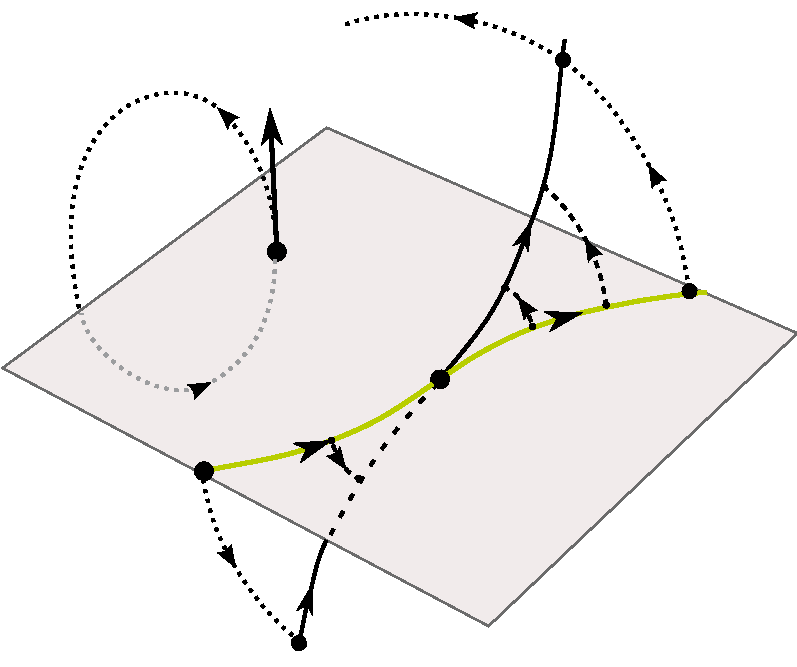
\includegraphics[width=\unitlength]{ReducTraj5}}%
   \put(0.06854399,0.36282057){\color[rgb]{0,0,0}\rotatebox{-30.34758661}{\makebox(0,0)[lb]{\smash{$\pSRed$}}}}%
   \put(0.57768586,0.29773425){\color[rgb]{0,0,0}\rotatebox{0.0313674}{\makebox(0,0)[lb]{\smash{$\sspRed(0)$}}}}%
   \put(0.59310014,0.69932675){\color[rgb]{0,0,0}\rotatebox{0.03136739}{\makebox(0,0)[lb]{\smash{$\ssp(\zeit)$}}}}%
   \put(0.8268425,0.39772328){\color[rgb]{0,0,0}\rotatebox{0.03136739}{\makebox(0,0)[lb]{\smash{$\sspRed(\zeit)$}}}}%
   \put(0.81220962,0.66529577){\color[rgb]{0,0,0}\rotatebox{0.03136739}{\makebox(0,0)[lb]{\smash{$\matrixRep(\theta(\zeit))\ssp(\zeit)$}}}}%
   %\put(0.21150193,0.63610779){\color[rgb]{0,0,0}\rotatebox{0.0313674}{\makebox(0,0)[lb]{\smash{$\matrixRep(\theta)\\slicep$}}}}%
   \put(0.37740434,0.49597258){\color[rgb]{0,0,0}\rotatebox{0.0313674}{\makebox(0,0)[lb]{\smash{$\slicep$}}}}%
   \put(0.3627714,0.69665188){\color[rgb]{0,0,0}\rotatebox{0.0313674}{\makebox(0,0)[lb]{\smash{$\sliceTan{}$}}}}%
 \end{picture}%
\end{center}
\caption{\label{f-ReducTraj1}
(Color online) The \slicePlane\ \pSRed\ is a hyperplane % \refeq{PCsect0}
passing through the {\template} point $\slicep$ and normal to its group
tangent $\sliceTan{}$. It intersects all group orbits (dotted lines) in
an open neighborhood of $\slicep$.  The full \statesp\ trajectory
$\ssp(\tau)$ (solid black line) and the \reducedsp\ trajectory
$\sspRed(\zeit)$ (solid green line) belong to the same group orbit
$\pS_{\ssp(\zeit)}$ and are equivalent up to a group rotation
$\matrixRep(\theta(\zeit))$.
}%
\end{figure}

Reduced trajectories $\sspRed (t)$ can be obtained in two ways: by
post-processing data or by reformulating the dynamics and integrating
directly in the \slice. The post-processing method (also called the
\emph{method of moving frames}\rf{FelsOlver98,OlverInv}) can be applied
to both numerical and experimental data, one takes the data in the full
\statesp\ and looks for the time dependent group parameter that brings
the trajectory $\ssp(\zeit)$ onto the \slice. That is, one finds $\theta
(\zeit)$ such that $\sspRed(\zeit)=\matrixRep(-\theta (\zeit)) \ssp
(\zeit)$ satisfies the \slice\ condition:
\beq
\braket{\sspRed(\zeit) - \slicep}{\sliceTan{}} = 0
\,.
\ee{SliceCond}

In the second implementation, one reformulates the dynamics (for Abelian
groups) as
\begin{subequations}\label{eq:so2reduced}
  \beq\label{eq:intSlice}
	\velRed(\sspRed) = \vel(\sspRed)
	-\dot{\theta}(\sspRed) \, \groupTan(\sspRed)
  \eeq
  \beq\label{eq:reconstruction}
	\dot{\theta}(\sspRed) = {\braket{\vel(\sspRed)}{\sliceTan{}}}/
				{\braket{\groupTan(\sspRed)}{\sliceTan{}}}
  \, ,
  \eeq
\end{subequations}
and directly calculates the symmetry-reduced trajectory directly by integrating $\sspRed (\zeit)$ and $\theta (\zeit)$.
In \refeq{eq:so2reduced}, $\velRed$ is the projection of the full \statesp\ velocity \vel(\ssp) onto the \slicePlane.
For a derivation of \refeq{eq:so2reduced}, see \refref{DasBuch}.

While early studies\rf{rowley_reconstruction_2000, rowley_reduction_2003,
BeTh04} applied the \mslices\ to a single solution at a time, studying
the nonlinear dynamics of extended systems requires symmetry reduction of
global objects, such as strange attractors or invariant manifolds. In
this spirit, Siminos and Cvitanovi\'{c}\rf{SiCvi10} used the \mslices\ to
quotient the \SOn{2} symmetry from the chaotic dynamics of \cLf. They
showed that the slice-dependent singularity of the reconstruction
equation that occurs when the denominator in \refeq{eq:reconstruction}
vanishes (e.g., when the group tangents of the trajectory and the
template are orthogonal) causes the reduced flow to make discontinuous
jumps. This set of points $\sspRed^*$ in the \slicePlane\ that satisfy
\beq
\braket{\groupTan(\sspRed^*)}{\sliceTan{}} = 0
\ee{ChartBordCond}
forms the \emph{\sliceBord}, studied in detail by Froehlich and Cvitanovi\'{c}\rf{FrCv11}.

Two strategies have been proposed in order to handle this problem: The first attempts to
try to identify a template such that slice singularities are not visited
by the dynamics\rf{SiCvi10} or to use multiple `charts' of connected
slices\rf{rowley_reconstruction_2000,FrCv11}.
The latter approach was applied to \cLf\ by Cvitanovi\'{c} \etal~\rf{atlas12} and
to pipe flow by Willis, Cvitanovi\'{c}, and Avila\rf{ACHKW11}.
However, neither approach is straightforward to apply, particularly in
high-dimensional dynamical systems.

\subsection{\FFslice}
\label{sect:fFslice}

A third strategy has recently been proposed by Budanur
\etal\rf{BudCvi14}, who considered Fourier space discretizations of
partial differential equations (PDEs) with \SOn{2} symmetry. They showed
that in these cases a simple choice of \slice\ template, associated with
the first Fourier mode, results in a \slice\ in which it is highly
unlikely that generic dynamics visit the neighborhood of the singularity.
If the dynamics do occasionally come near the singularity, these close
passages can be regularized by means of a time rescaling.

Here, we shall illustrate this approach, which we call the `\fFslice',
and apply it to a 2-mode model system described in \refsect{s:twoMode},
arguably the simplest system with \SOn{2} equivariant dynamics that can
exhibit chaos.

In the discussion so far, we have not specified any constraints on the 
symmetry group to be quotiented, beyond the requirement that it be Abelian, 
which is required for \refeq{eq:so2reduced} to be valid. Since we are 
interested in spatially extended systems with translational symmetry, and in 
order to keep the notation compact, we restrict our discussion to one 
dimensional PDEs describing the evolution of a field $u(x,t)$ in a periodic 
domain. By introducing a Fourier series expansion
\beq
	u(x,\zeit) = \sum\limits_{k=- \infty}^\infty u_k\left(\zeit\right) 
				 e^{i k x}, \,\,\,u_k = x_k + i y_k,
\ee{FourierSeries}
a PDE invariant under translations can be expressed as a system of coupled 
nonlinear ODEs equivariant under the 1-parameter compact group of \SOn{2} 
rotations.

Truncating the expansion to $m$ modes, we write the real and imaginary parts 
of the Fourier coefficients with $k \geq 1$ as the state vector 
$\ssp=\cartpt{x_1, y_1, x_2, y_2,..., x_m, y_m}$. The action of the $\SOn{2}$ 
group on this vector can then be expressed as a block diagonal matrix:
\beq
	\matrixRep(\theta) = \begin{pmatrix}
						R(\theta) & 0 			  & \cdots & 0 \\
						0		   & R(2 \theta) & \cdots & 0 \\
						\vdots	   & \vdots 	  & \ddots & \vdots \\
						0		   & 0	          & \cdots & R (m \theta)
					   \end{pmatrix}
\,,
\ee{mmodeLieEl}
where
\beq
	R(n \theta) =	\begin{pmatrix}
					\cos n \theta & - \sin n \theta \\
					\sin n \theta & ~\cos n \theta
					\end{pmatrix}
\ee{rotationmatrix}
is the rotation matrix for $n$th Fourier mode.
The Lie algebra generator for $\matrixRep(\theta)$ is given by
\beq
	 \Lg =  \begin{pmatrix}
			 0 & -1 & 0 & 0 & \cdots & 0 & 0 \\
			 1 & 0 & 0 & 0 & \cdots & 0 & 0 \\
			 0 & 0 & 0 & -2 & \cdots & 0 & 0 \\
			 0 & 0 & 2 & 0 & \cdots & 0 & 0 \\
			 \vdots & \vdots & \vdots & \vdots & \ddots & \vdots & \vdots \\
			 0 & 0 & 0 & 0 & \cdots & 0 & -m \\
			 0 & 0 & 0 & 0 & \cdots & m & 0
			 \end{pmatrix} .
\ee{mmodeLg}

In order to construct a \slicePlane\ for such a system, let us choose the
following \slice\ \template:
\beq
	\slicep = (1, 0, ..., 0) .
\ee{firstmodetemp}
The \slice\ condition \refeq{SliceCond} then constraints points on the
reduced trajectory to the hyperplane given by
\beq
	\sspRed = (\hat{x}_1, 0, \hat{x}_2, \hat{y}_2, ..., \hat{x}_m, \hat{y}_m) .
\ee{slicetemp}
As discussed earlier, group orbits should cross the \slice\ once and only
once, which we achieve by restricting the \slicePlane\ to the half-space
where $\hat{x}_1 > 0$. In general, a \slicePlane\ can be constructed by
following a similar procedure for any choice of \template, allowing the
symmetry reduction of the dynamics in a neighborhood of the \template\
bounded by the \sliceBord\ \refeq{ChartBordCond}. However, the power of
choosing template \refeq{firstmodetemp} becomes apparent by computing the
border of its \slicePlane. The points on \refeq{slicetemp} lie on the
\sliceBord\ only if $\hat{x}_1 = 0$. This means that as long the dynamics
are such that the magnitude of the first mode never vanishes,
\emph{every} group orbit is guaranteed to have a unique representative
point on the \slicePlane. By symmetry, any template of the form $\slicep
=\cartpt{\hat{x}'_1, \hat{y}'_1, 0,...,0}$  would work just as well. The
\slice\ \template\ \refeq{firstmodetemp} was chosen for notational and
computational convenience.

More insight can be
gained by writing the symmetry-reduced evolution equations 
\refeq{eq:so2reduced} explicitly for the template \refeq{firstmodetemp}:
\begin{subequations}
\beq
\velRed ( \sspRed )  = \vel(\sspRed)
   - \frac{\dot{y}_1\left(\sspRed\right)}{\hat{x}_1} \, \groupTan(\sspRed) \, ,
\label{e-so2red1stmode}
\eeq
\ESedit{
  \beq\label{eq:reconstruction1stmode}
	\dot{\theta}(\sspRed) = \frac{\dot{y}_1(\sspRed)}{\hat{x}_1}
  \, .
  \eeq
}
\end{subequations}
Since the argument $\phi_1$ of a point $(x_1,y_1)$ in the first Fourier mode 
plane is given by $\phi_1=\tan^{-1}\frac{y_1}{x_1}$, its velocity is
\beq
  \dot{\phi}_1 = \frac{x_1}{r_1^2}\dot{y}_1-\frac{y_1}{r_1^2}\,\dot{x}_1\,,
\eeq
where $r_1^2=x_1^2+y_1^2$. Therefore, on the \slicePlane \refeq{slicetemp}, 
where $\hat{y}_1=0$,
\beq\label{eq:phi1}
  \dot{\theta}(\sspRed) = \dot{\phi}_1(\sspRed)\,.
\eeq
That is, for our choice of \template\ \refeq{firstmodetemp}, the
reconstruction phase coincides with the first Fourier mode phase. In this
sense, from a group-theoretic point of view, this choice of template is
thus more natural than the physically motivated templates used in
\refrefs{rowley_reconstruction_2000,BeTh04,SiCvi10,FrCv11,atlas12,ACHKW11}.

In general, additional care must be taken when the dynamics approach the 
\slice\ border $\hat{x}_1 = 0$. Whenever this happens, the near-divergence of 
$\velRed$ can be regularized by introducing a rescaled time coordinate such 
that $d\hat{\zeit} = d\zeit / \hat{x}_1$\rf{BudCvi14}. However, in our study 
of the \twomode\ system that we will introduce below, we omit this step since 
points with a vanishing first mode are in an invariant subspace of the flow 
and hence are never visited by the dynamics.

\subsection{Post-processing approach}
\label{s-mframes}

\begin{figure}%[H]
\centering
 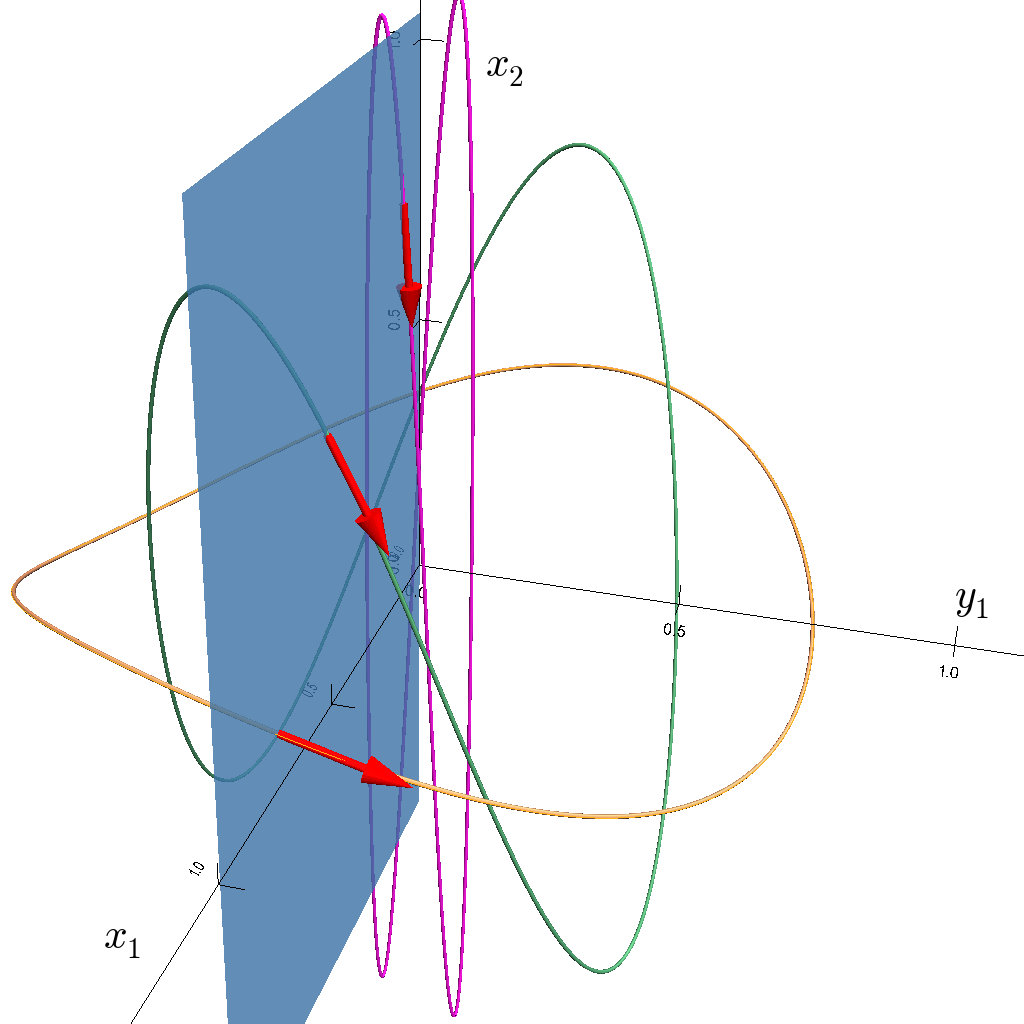
\includegraphics[width=0.45\textwidth]{BBgorbitsandslice}
\caption{(Color online)
$\SOn{2}$ group orbits of \statesp\ points $\cartpt{0.75, 0, 0.1, 0.1}$
(orange), $\cartpt{0.5, 0, 0.5, 0.5}$ (green)
$\cartpt{0.1, 0, 0.75, 0.75}$ (pink) and the first mode \refeq{slicetemp} 
\slicePlane\ (blue). The group tangents at the intersections with the
\slicePlane\ are shown as red arrows.
As the magnitude of the first Fourier mode decreases relative to the
magnitude of the second one, so does the group tangent angle to the
\slicePlane.}
\label{fig:BBgorbitsandslice}
\end{figure}

In \refsect{s-slice}, we explained the general procedure for reducing the 
\SOn{2} symmetry by \mslices. Here, we focus on its geometrical 
interpretation. The \slice\ defined by \refeq{firstmodetemp} and the 
directional constraint $\hat{x}_1 > 0$ fixes the phase of the first complex 
Fourier mode to $0$. This also follows from the fact that the reconstruction 
phase of the first Fourier mode \slice\ is the phase of the first mode 
In complex representation, we can express the relationship between Fourier 
modes ($\sspC_n = x_n + \ii y_n$) and their representative points 
($\sspRedC = \hat{x}_n +  \ii \hat{y}_n$) on the \slicePlane\ by the $\Un{1}$ 
action:
\beq
	\sspRedC_n = e^{-\ii n \phi_1} \sspC_n \, . \ee{e-1stmodeTransform}
This relation provides another interpretation for the \sliceBord:  For
template \refeq{firstmodetemp}, the \sliceBord\ condition
\refeq{ChartBordCond} yields, $|\sspRedC_1| = |\sspC_1| = 0$, which means
that the phase of the first Fourier mode and hence the
transformation \refeq{e-1stmodeTransform} is not well-defined.
This is illustrated in \reffig{fig:BBgorbitsandslice}, which shows the
first Fourier mode \slicePlane\ along with three-dimensional projections
of the group orbits of points with decreasing $|\sspC_1|$. When the
magnitude of the first mode $\sqrt{\hat{x}_1^2 + \hat{y}_1^2}$, relative
to that of the second mode is small (pink curve in
\reffig{fig:BBgorbitsandslice}), the group tangent has a larger component
parallel to the \slicePlane . If the first mode magnitude was exactly
$0$, the group tangent would lie entirely on the \slicePlane , satisfying
the \sliceBord\ condition.

In \refref{PoKno05}, a polar coordinate representation of two Fourier mode
truncation is obtained by defining the $\Group$-invariant phase: 
$\Phi = \phi_2 - 2 \phi_1$
and three symmetry invariant coordinates 
\polpt{r_1, r_2 \cos \Phi, r_2 \sin \Phi}.
One can see by direct comparison with \refeq{e-1stmodeTransform}, which
yields $\sspRedC_1 = r_1$ and $\sspRedC_2 = r_2 e^{\ii \Phi}$, that this
representation is a special case $(m=2)$, of the \slice\ defined by
\refeq{firstmodetemp}. Corresponding ODEs for the polar representation
were obtained in \refref{PoKno05} by  chain rule and substitution. Note
that \mslices\ provides a general form \refeq{e-so2red1stmode} for symmetry
reduced time evolution.

\section{\twoMode\ $\SOn{2}$-equivariant flow}
\label{s:twoMode}

Dangelmayr,\rf{Dang86} Armbruster, Guckenheimer and Holmes,\rf{AGHO288}
Jones and Proctor,\rf{JoPro87} and Porter and Knobloch\rf{PoKno05} (see
Golubitsky \etal\rf{golubII}, Sect. XX.1) have investigated bifurcations
in 1:2 resonance ODE normal form models to third order in the amplitudes.
Here, we use this model as a starting point from which we derive what may
be one of the simplest chaotic systems with a continuous symmetry. We refer 
to this as the {\twomode} system:
\bea
	\dot{z}_1 &=& (\mu_1-\ii\, e_1)\,z_1+a_1\,z_1|z_1|^2
				 +b_1\,z_1|z_2|^2+c_1\,\overline{z}_1\,z_2
	\continue
	\dot{z}_2 &=& (\mu_2-\ii\, e_2)\,{z_2}+a_2\,z_2|z_1|^2
				 +b_2\,z_2|z_2|^2+c_2\,z_1^2 \,,
	\label{eq:DangSO2}
\eea
where $z_1$ and $z_2$ are complex and all parameters real-valued. The 
parameters $\{e_1,e_2\}$ break the $\On{2}$ symmetry of the normal form 
studied by Dangelmayr\rf{Dang86} leading to an $\SOn{2}$-equivariant system. 
As we will show below in \refeq{PKinvEqs1}, only the combination $(2e_1-e_2)$ 
matters in the symmetry reduced dynamics, so for simplicity we set $e_1=0$. 
This complex two mode system can be expressed as a 4-dimensional first order 
real ODE system by substituting $z_1 = x_1 + i\,y_1$, $z_2 = x_2 + i\,y_2$, 
so that 
\bea
\dot{x}_1 &=& (\mu_1 + a_1 r_1^2 + b_1 r_2^2 + c_1 x_2)x_1 
			  + c_1 y_1 y_2 + e_1 y_1 \, ,
\continue
\dot{y}_1 &=& (\mu_1 + a_1 r_1^2 + b_1 r_2^2 - c_1 x_2)y_1 
			  + c_1 x_1 y_2 - e_1 x_1 \, ,
\continue
\dot{x}_2 &=& (\mu_2 + a_2 r_1^2 + b_2 r_2^2)x_2 
			  + c_2 (x_1^2 - y_1^2) + e_2 y_2 \, ,
\label{2mode4D}
\continue
\dot{y}_2 &=& (\mu_2 + a_2 r_1^2 + b_2 r_2^2)y_2 
			  + 2 c_2 x_1 y_1 - e_2 x_2 \, ,
\continue
		  && \mbox{where } r_1^2 = x_1^2 + y_1^2\, , \quad r_2^2 = x_2^2 + y_2^2
\,.
\eea
This normal form has a large set of parameters 
$\left(\mu_1,\mu_2,a_1,a_2,b_1,b_2,c_1,c_2,e_1,e_2\right)$. Following in the 
tradition of Lorenz\rf{lorenz}, H\'enon\rf{henon} and R\"ossler\rf{ross}, we 
have played with various choices of parameters until settling on the following 
set of values, which we will use in all numerical calculations presented here:
\beq
	\begin{tabular}{c c c c c c c c c c}
	 $\mu_1$ & $\mu_2$ & $e_1$ & $e_2$ & $a_1$ & $a_2$ & $b_1$ & $b_2$ & $c_1$ & $c_2$ \\
	\hline
	 -2.8	& 1		  & 0	  & 1	  & -1	  & -2.66 & 0	  & 0 	  & -7.75 & 1
	\end{tabular}
	\label{eq:pars}
\eeq
This choice of parameters is far from the bifurcation values studied by 
previous authors\rf{Dang86,AGHO288,JoPro87,PoKno05}, so that the model has no 
physical interpretation. However, this set of parameters yield chaotic 
dynamics, making the two-mode system a simple model for the study of chaos in 
the presence of a continuous symmetry: It is a 4\dmn\ $\SOn{2}$-equivariant 
model in which the three dimensional $\SOn{2}$-reduced dynamics are chaotic.

It can be checked by inspection that eqs.~\refeq{eq:DangSO2} are equivariant 
under the \Un{1}\ transformation
\beq
(z_1,z_2) \rightarrow   (e^{i {\gSpace}}z_1,e^{i 2{\gSpace}} z_2)
\,.
\ee{Dang86(1.1)aa}
In the real representation \refeq{2mode4D}, the $\SOn{2}$ group action
\refeq{Dang86(1.1)aa} is given by $\ssp'= \exp\left( \theta \Lg\right)\ssp$,
where $\transp{\ssp} =\cartpt{x_1, y_1,x_2, y_2}$, and $\Lg$ is the Lie algebra
generator
\beq
\Lg  \, =
\left( \begin{array}{cccc}
         0 & -1 & 0 & 0 \\
         1 & 0 & 0 & 0 \\
         0 & 0 & 0 & -2\\
         0 & 0 & 2 & 0
      \end{array} \right)
\,.
\ee{LGTwoMode}
One can easily check that the real \twomode\ system \refeq{2mode4D}
satisfies the equivariance condition \refeq{inftmInv}.

From \refeq{eq:DangSO2}, it is obvious that the \eqv\ point \((z_1,z_2)=(0,0)\)
is an invariant subspace, and that $z_1=0$, $z_2 \neq 0$ is a 2\dmn\
flow-invariant subspace,
\beq
  \dot{z}_1 = 0 
\,,\qquad
  \dot{z}_2 = (\mu_2-\ii\, e_2 +b_2 |z_2|^2)\,{z_2} 
\,,
\ee{eq:DangSO2spsp}
with a single circular \reqv\ of radius 
$r_2 = \norm{z_2} = \sqrt{-\mu_2/b_2}$ with \phaseVel\ $\velRel=-e_2/2$. At 
the origin the stability matrix $\Mvar$ commutes with $\Lg$, and thus can be 
block-diagonalized into two $[2\!\times\!2]$ matrices. The eigenvalues of 
$\Mvar$ at $\cartpt{0,0,0,0}$ are $\Lyap_1 = \mu_1$ with multiplicity 2 and
$\Lyap_2 = \mu_2 \pm i e_2$. The eigenvectors for $\Lyap_1$ are 
$\cartpt{1,0,0,0}$ and $\cartpt{0,1,0,0}$ in the $\cartpt{x_1,y_1,x_2,y_2}$ 
coordinates. The eigenvectors for $\Lyap_2$ are $\cartpt{0,0,1,0}$ and 
$\cartpt{0,0,0,1}$.

In contrast, $z_2 =0$ is not, in general, a flow-invariant subspace, since the dynamics
\[
  \dot{z}_1 = (\mu_1-\ii\, e_1)\,z_1+a_1\,z_1|z_1|^2
\,,\qquad
  \dot{z}_2 = c_2\,z_1^2
\,.
\]
takes the flow out of the $z_2 =0$ plane.

\subsection{Invariant polynomial bases}
\label{s:invPol}

Consider the \statesp\ of a dynamical system constructed from two complex
Fourier modes\rf{Dang86,AGHO288,PoKno05} $m=(1,2)$, with the $\SOn{2}
\simeq \Un{1}$ group action given by \refeq{Dang86(1.1)aa}. In this case,
it is easy to construct a set of four real-valued $\SOn{2}$ invariant
polynomials
\bea
u &=& {z}_1 \overline{z}_1
    \,,\quad
v = {z}_2 \overline{z}_2
    \continue
w &=& z_1^2 \overline{z}_2 + \overline{z}_1^2 {z}_2
    \,,\quad
q = (z_1^2 \overline{z}_2 - \overline{z}_1^2 {z}_2)/\ii
\,.
\label{Dang86(1.2)PK}
\eea
The polynomials $\invpt{u,v,w,q}$ are linearly independent, but related 
through one syzygy,
\beq
w^2+q^2 - 4\,u^2v = 0 
\label{eq:syzPK}
\eeq
that confines the dynamics to a 3-dim\-ens\-ion\-al manifold 
$\pSRed=\pS/\SOn{2}$, a symmetry-invariant repre\-sent\-ati\-on of the 
4-dim\-ens\-ion\-al \SOn{2} equivariant dynamics, which we call the 
\reducedsp. By construction, $u \geq 0$, $v \geq 0$, but $w$ and $q$ can be of 
either sign. That is explicit in in polar coordinates 
$ {z}_1 = |u|^{1/2} e^{\ii\phi_1}$, $ {z}_2 = |v|^{1/2} e^{\ii\phi_2}$, where 
the  $w, q$ invariants take the form
\bea
w &=& 2\,\Re(z_1^2 \overline{z}_2) = 2\,u |v|^{1/2} \cos \psi 
\continue
q &=& 2\,\Im(z_1^2 \overline{z}_2) = 2\,u |v|^{1/2} \sin \psi 
\,,
\label{Dang86(1.2)polar}
\eea
where $\psi = 2 \phi_1 - \phi_2$.

The dynamical equations for $\invpt{u,v,w,q}$ follow from the chain rule, which yields
\bea
  \dot{u} &=& \overline{z}_1 \dot{z}_1 + {z}_1 \dot{\overline{z}}_1 
\,,\qquad
  \dot{v} = \overline{z}_2 \dot{z}_2 + {z}_2 \dot{\overline{z}}_2 
\continue
  \dot{w} &=& 2 \,\overline{z}_2 {z}_1 \dot{z}_1 
           + 2\,{z}_2 \overline{z}_1 \dot{\overline{z}}_1
           + {z}_1^2 \dot{\overline{z}}_2
           + \overline{z}_1^2 \dot{z}_2
\continue
  \dot{q} &=&  (2\,\overline{z}_2 {z}_1 \dot{z}_1 
           - 2\,{z}_2 \overline{z}_1 \dot{\overline{z}}_1
           + {z}_1^2 \dot{\overline{z}}_2
           - \overline{z}_1^2 \dot{z}_2
           )/\ii
\label{PKinvEqs}
\eea
Substituting \refeq{eq:DangSO2} into \refeq{PKinvEqs}, we obtain a set of four 
$\SOn{2}$-invariant equations,
\bea
  \dot{u} &=& 2\,\mu_1\,u+2\,a_1\,u^2+2\,b_1\,u\,v+c_1\,w 
\continue
  \dot{v} &=& 2\,\mu_2\,v+2\,a_2\,u\,v+2\,b_2\,v^2+c_2\,w 
\continue
  \dot{w} &=& (2\,\mu_1+\mu_2)\,w+(2a_1+a_2)\,u\,w+(2b_1+b_2)\,v\,w 
\ceq
             +\, 4c_1\,u\,v + 2c_2\,u^2 +(2e_1 - e_2)\,q
\label{PKinvEqs1}\\
  \dot{q} &=& (2\mu_1+\mu_2)\,q+(2a_1+a_2)\,u\,q
\ceq
             +(2b_1+b_2)\,v\,q
             -(2e_1-e_2)\,w 
\,.
\nnu
\eea
Note that the $\On{2}$-symmetry breaking parameters $\{e_1,e_2\}$ of the
Dangelmayr normal form system\rf{Dang86} appear only in the relative phase 
combination $(2e_1-e_2)$. Using the syzygy \refeq{eq:syzPK}, we can eliminate 
$q$ from \refeq{PKinvEqs1} to get
\bea
  \dot{u} &=& 2\,\mu_1\,u+2\,a_1\,u^2+2\,b_1\,u\,v+c_1\,w \nonumber 
\\
  \dot{v} &=& 2\,\mu_2\,v+2\,a_2\,u\,v+2\,b_2\,v^2+c_2\,w \label{PKinvEqs1syz}  
\\
  \dot{w} &=& (2\,\mu_1+\mu_2)\,w+(2a_1+a_2)\,u\,w+(2b_1+b_2)\,v\,w 
\ceq
             +\, 4c_1\,u\,v + 2c_2\,u^2 +(2e_1 - e_2)(4u^2v-w^2)^{1/2}\,
  \nonumber
\eea
This invariant basis can be used either to investigate the dynamics directly 
or to visualize solutions\rf{GL-Gil07b} computed in the full equivariant basis 
\refeq{eq:DangSO2}. While representations of our model in terms of invariant 
polynomials \refeq{PKinvEqs1} and polar coordinates \refeq{Dang86(1.2)polar} 
are useful for cross-checking calculations in the full \statesp\ 
$\transp{\ssp} =\cartpt{x_1, x_2,y_1, y_2}$ , construction requires a bit of 
algebra even for this simple 4-dimensional flow. For very high\dmn\ flows, 
such as \KS\ and \NS\ flows, we do not know how to carry out such 
constructions.

\subsection{\Eqva\ of the symmetry-reduced dynamics}
\label{s:eqva}

The first step in elucidating the geometry of attracting sets is the
determination of their \eqva. We shall now show that the problem of
determining the \eqva\ of the symmetry-reduced \twomode\
\refeq{PKinvEqs1} system $\invpt{u^*,v^*,w^*,q^*}$ can be reduced to
finding the real roots of a multinomial expression. First, let we define
\beq
A_1= \mu_1+a_1\,u+b_1\,v
    \,,\qquad
A_2 = \mu_2+a_2\,u+b_2\,v
\ee{PKinvEqs2a}
and rewrite \refeq{PKinvEqs1} as
\bea
  0  &=&  2\,A_1\,u +c_1\,w 
    \,,\qquad
  0  =  2\,A_2\,v +c_2\,w 
\continue
  0  &=& (2\,A_1+ A_2)\,w
          +2\,\left(c_2\,u+2\,c_1\,v\right)\,u 
          \ceq
		  + (2e_1-e_2)\,q
\label{PKinvEqs3}\\
  0  &=& (2\,A_1+ A_2)\,q - (2e_1-e_2)\,\,w 
\nnu
\eea
We already know that $\invpt{0,0,0,0}$ and $\cartpt{0,-\mu_2/b_2,0,0}$ are the 
only roots in the $u=0$ and $v=0$ subspaces, so we are looking only for the 
$u>0$, $v>0$, $w,q \in \reals$ solutions; there could be non-generic roots 
with either $w=0$ or $q=0$, but not both simultaneously, since the syzygy 
\refeq{eq:syzPK} precludes that. Either $w$ or $q$ can be eliminated by 
obtaining the following relations from \refeq{PKinvEqs3}:
\bea
	w  &=& - \frac{2\,u}{c_1}\,A_1 = - \frac{2\,v}{c_2}\,A_2 
	\continue
	q &=& \frac{2(-2e_1+\,e_2)\,u\,v}{c_2\,u+2\,c_1\,v} .  root.
	\label{PKinvEqs4}
\eea
Substituting \refeq{PKinvEqs4} into \refeq{PKinvEqs3} we get two bivariate
polynomials whose roots are the \eqva\ of the system \refeq{PKinvEqs1}:
\bea
	f(u,v) &=& c_2\,u\,A_1 - c_1\,v\,A_2 = 0 \,,\qquad  \nonumber
	\\
	g(u,v) &=&
 \left(4\,A_1^2 u^2 - 4\,c_1^2\,u^2 v\right)\left(c_2\,u+2\,c_1\,v\right)^2 \label{PKinvEqs5} 
	\ceq
	+\,4\,c_1^2\,(-2e_1+e_2)^2\,u^2\,v^2 = 0
\,,
	\\
	\mbox{\rm deg}(f) &=& 2, \, \mbox{\rm deg}(g) = 6 \nonumber
\,.
\eea
We divide the common multiplier $u^2$ from the second equation and by doing 
so, eliminate one of the two roots at the origin, as well as the 
$\cartpt{0,-\mu_2/b_2,0,0}$ root within the invariant subspace
\refeq{eq:DangSO2spsp}. Furthermore, we scale the parameters and variables as
$\tilde{u} = c_2\,u$,
$\tilde{v} = c_1\,v$,
$\tilde{a_1} = a_1/c_2$,
$\tilde{b_1} = b_1/c_1$,
$\tilde{a_2} = a_2/c_2$,
$\tilde{b_2} = b_2/c_1$
to get
\bea
\tilde{f}(\tilde{u},\tilde{v}) &=&
  \tilde{u}\,\tilde{A}_1 - \tilde{v}\,\tilde{A}_2 = 0 
\,,\qquad \mbox{\rm deg}(f) = 2 \, , \label{PKinvEqs5a}
\\
\tilde{g}(\tilde{u},\tilde{v}) &=&  
 \left(\tilde{A}_1^2
 - c_1\,\tilde{v}\right)
 \left(\tilde{u}+2\,\tilde{v}\right)^2
 +e_2^2\,\tilde{v}^2 = 0
\,,
\ceq
   \mbox{\rm deg}(g) = 4 \, , \label{PKinvEqs5b}
\\
 && \mbox{where }
\tilde{A}_1 = \mu_1+\tilde{a_1}\,\tilde{u}+\tilde{b_1}\,\tilde{v}
\,,\ceq
\qquad\quad \tilde{A}_2 = \mu_2+\tilde{a_2}\,\tilde{u}+\tilde{b_2}\,\tilde{v}
\,,
\label{PKinvEqs5c}
\eea
Solving coupled bivariate polynomials \refeq{PKinvEqs5a} is not, in general, a 
trivial task. However, for the choice of parameters given by \refeq{eq:pars}, 
eq.~\refeq{PKinvEqs5a} yields 
$\tilde{v} = (\mu_1 + \tilde{a}_1 \tilde{u})/(\mu_2 + \tilde{a}_2 \tilde{u})$. 
Substituting this into \refeq{PKinvEqs5b} makes it a fourth order polynomial 
in $u$, which we can solve. Only the non-negative, real roots of this 
polynomial correspond to \reqva\ in the \twomode\ \statesp\ since $u$ and $v$ 
are the squares of first and second mode amplitudes, respectively. Two roots 
satisfy this condition, the \eqv\ at the origin:
\beq
	\invpol_{\EQV{}} = \invpt{0,0,0,0}\,, 
\ee{eq:origin}
and the \reqv:
\beq
	\invpol_{\REQV{}{}} = \invpt{0.193569,0.154131,-0.149539,-0.027178}\,.
\ee{eq:reqv}
Note that by setting $b_2 = 0$, we send the \reqv\ at
$\cartpt{0,-\mu_2/b_2,0,0}$ to infinity. Thus, \refeq{eq:reqv} is the
only \reqv\ of the \twomode\ system for our choice of parameters. While
this is an \eqv\ in the invariant polynomial basis, in the
\SOn{2}-equivariant, real-valued \statesp\ this is a 1\dmn\ \reqv\ group orbit.
The point on this orbit that lies in first Fourier mode slice is
(see \refFig{fig:2modes-ssp}\,(c)):
\beq
  \left(x_1, y_1, x_2, y_2\right) = \left(0.439966, 0, -0.386267, 0.070204\right)
\,.
  \label{e-req}
\eeq
We computed the linear stability eigenvalues and eigenvectors of this \reqv
, by evaluating \stabmat\ within the first Fourier mode slice
$\MvarRed_{ij} (\sspRed) = \partial \velRed_i / \partial \sspRed_j |_{\sspRed}$
on the \reqv . Linear stability eigenvalues for the \reqv\ \refeq{e-req}
\beq
	\lambda_{1,2} = 0.05073 \pm \ii \, 2.4527, \quad
	\lambda_3 = -5.5055, \quad \lambda_4 = 0 \, .
\eeq
The $0$ eigenvalue corresponds to the direction outside the slice, we expect
this since the reduced trajectory equations \refeq{eq:intSlice} keeps the
solution within the slice. Imaginary part of the expanding complex pair sets
the `winding time' in the neighborhood of the equilibrium to
$T_w = 2 \pi / \Im(\lambda_1) = 2.5617$. The large \eqv\  of the
contracting eigenvalue $\lambda_3$ yields a very thin attractor in the
reduced \statesp, thus, when looked at on a planar Poincare\'{e} section,
the \twomode\ flow is almost one dimensional, see \reffig{fig:psectandretmap}\,(a, b).

\begin{figure*}%[H]
\centering
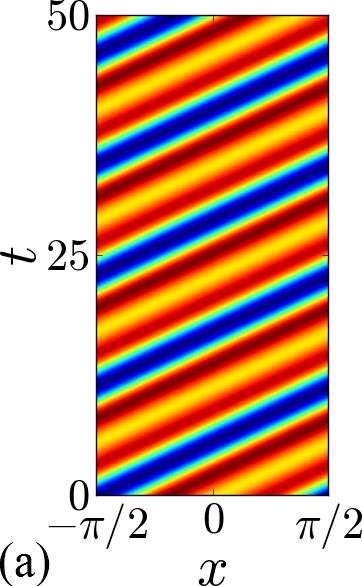
\includegraphics[height=0.22\textwidth]{2modes-conf-reqv}\quad%
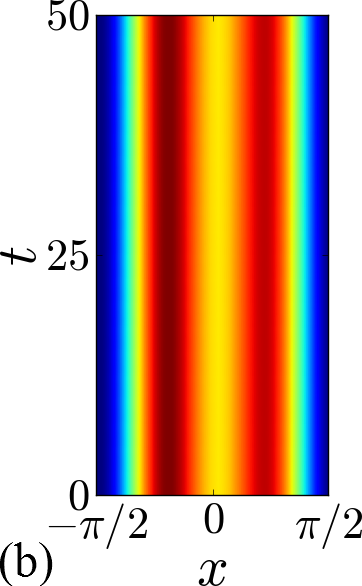
\includegraphics[height=0.22\textwidth]{2modes-confred-reqv}\quad%
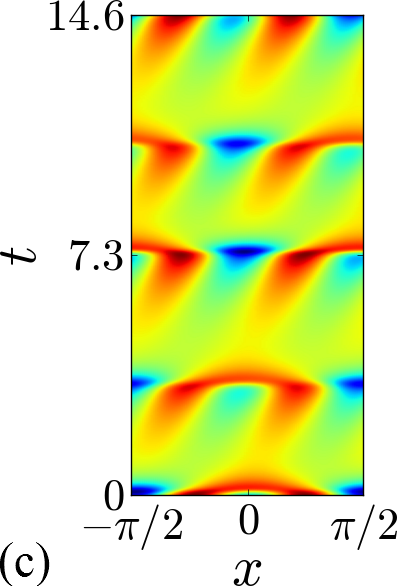
\includegraphics[height=0.22\textwidth]{2modes-conf-rpo}\quad%
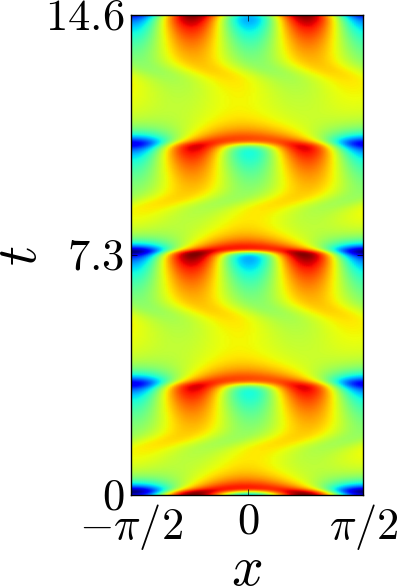
\includegraphics[height=0.22\textwidth]{2modes-confred-rpo}\quad%
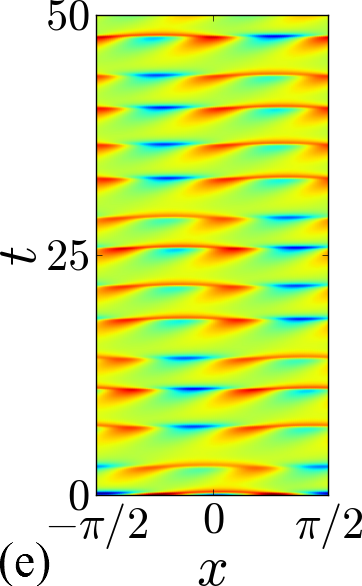
\includegraphics[height=0.22\textwidth]{2modes-conf-ergodic}\quad%
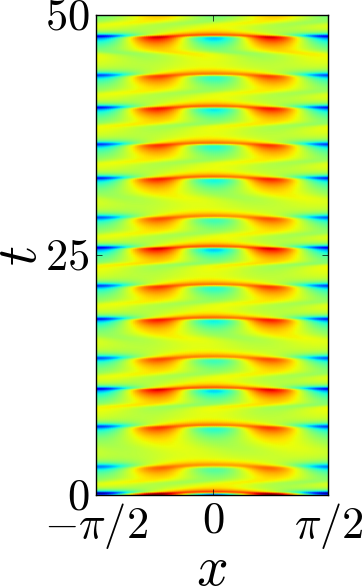
\includegraphics[height=0.22\textwidth]{2modes-confred-ergodic}%
\caption{(Color online)
The \reqv\ \REQV{}{} in
 (a) the system's configuration space becomes an \eqv\ in
 (b) the symmetry-reduced configuration space.
Two cycles of the \rpo\ \cycle{01} in the
 (c) the symmetry-equivariant configuration space become a \po\ in
 (d) the symmetry-reduced configuration space. A typical ergodic trajectory of 
 the \twomode\ system in the system's configuration space (e), in the 
 symmetry-reduced configuration space (f). The color scale used in each figure 
 is different to enhance contrast.
}
\label{fig:2modes-conf}
\end{figure*}

\begin{figure*}%[H]
\centering
(a)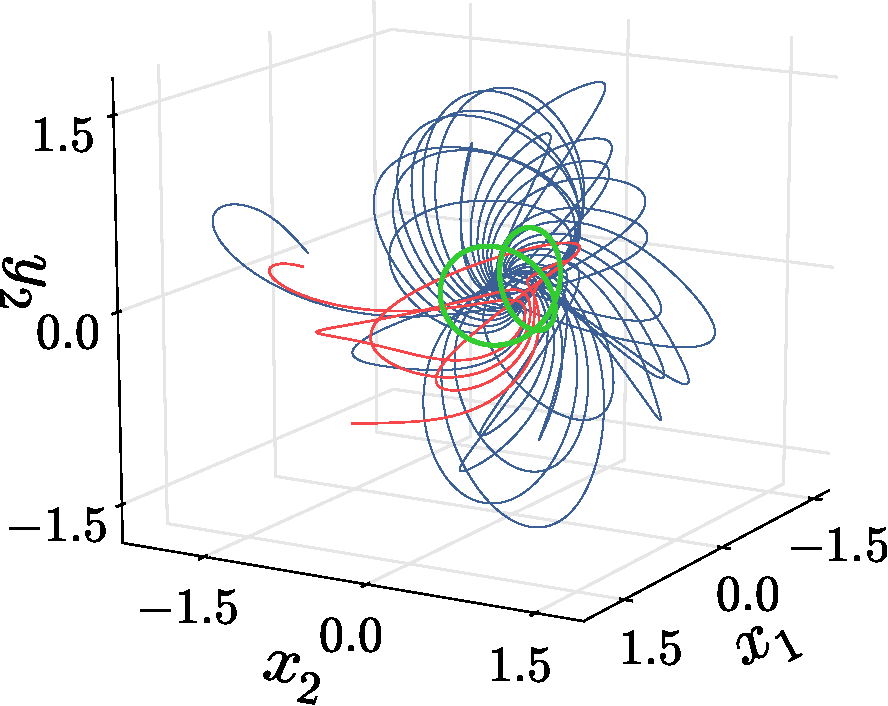
\includegraphics[width=0.30\textwidth]{2modes-ssp}
(b)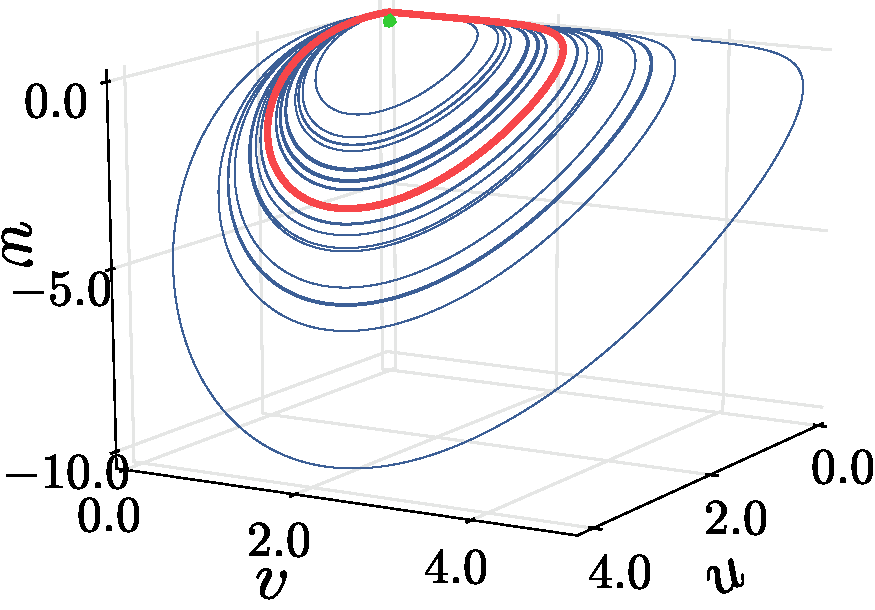
\includegraphics[width=0.30\textwidth]{2modes-invpol}
(c)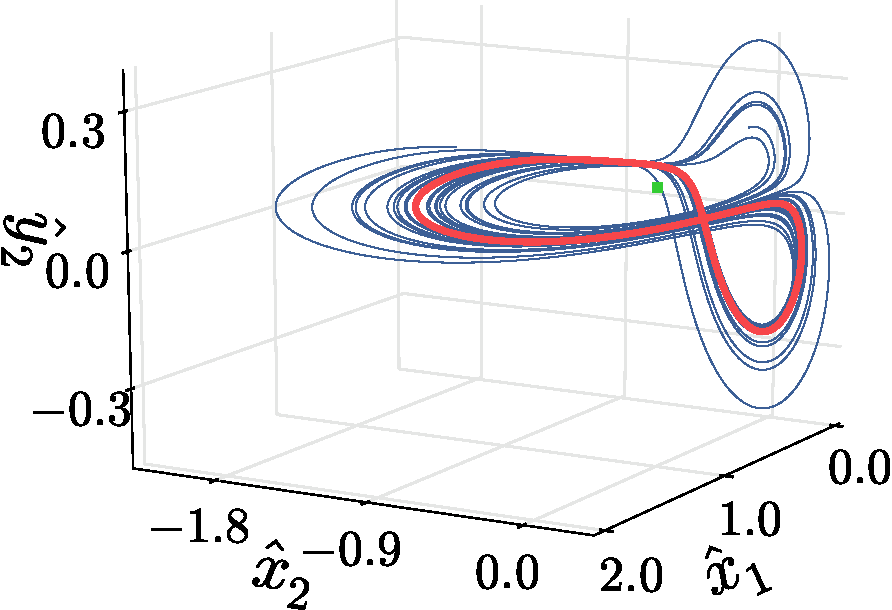
\includegraphics[width=0.30\textwidth]{2modes-sspRed}
\caption{(Color online)
The same trajectories as in \reffig{fig:2modes-conf}\,(a,c,d),
colored green, red and blue respectively,
	(a) in a 3D projection of the 4\dmn\ \statesp ,
	(b) in a terms of 3 invariant polynomials,
	(c) in the 3\dmn\  first Fourier mode \slicePlane.
Note that in the symmetry reduced representations (b and c), the \reqv\ 
\REQV{}{} is reduced to an \eqv , the green point; and the \cycle{01} (red) 
closes onto itself after one repeat. In contrast to the invariant polynomial 
representation (b), in the first Fourier mode \slicePlane (c), the qualitative 
difference between shifts by $\approx \pi$ and $\approx-\pi$ in near passages 
to the {\sliceBord} is very clear, and it leads to the unimodal Poincar\'e 
return map of \reffig{fig:psectandretmap}.
}
\label{fig:2modes-ssp}
\end{figure*}

\subsection{No chaos when the reflection symmetry is restored}
\label{s:dfsafs}

Before finishing our discussion of invariant polynomials, we make an important 
observation regarding the case when both of the reflection symmetry breaking
parameters, $e_{1}$ and $e_2$ are set to $0$. In this case, 
$\sspC_{1,2} \rightarrow \bar{\sspC}_{1,2}$ symmetry is restored and the 
evolution equations for $u$, $v$, and $w$ in \refeq{PKinvEqs1} become 
independent of $q$. Furthermore, the time evolution equation for $q$ becomes 
linear in $q$ itself, so that it can be expressed as:
\beq
    \dot{q} = \xi (u, v) q \,.
\ee{e-qlinearq}
Hence, the time evolution of $q$ can be written as
\beq
    q(\zeit) =  e^{\int_0^\zeit d \zeit' \xi (u(\zeit'), v(\zeit'))} q(0) \, .
\ee{e-qO2solq}
If we assume that the flow is bounded, then we can also assume that a long 
time average of $\xi$ exists. The sign of this average determines the long 
term behavior of $q(\zeit)$; it will either diverge or vanish depending on the 
sign of $\langle \xi \rangle$ being positive or negative respectively. The 
former case leads to a contradiction: If $q(\zeit)$ diverges, the 
symmetry-invariant flow cannot be bounded since the syzygy \refeq{eq:syzPK} 
must be satisfied at all times. If $q(t)$ vanishes, there are three invariant 
polynomials left, which are still related to each other by the syzygy. Thus, 
the flow is confined to a two dimensional manifold and cannot exhibit chaos.
We must stress that this is a special result which holds for the two-mode 
normal form with terms up to third order.

\subsection{Visualizing \twomode\ dynamics}
\label{s:visual}

We now present visualizations of the dynamics of the \twomode\ system in
four different representations: as 3D projections of the four-dimensional
real-valued \statesp, as 3D projections in the invariant polynomial
basis, as dynamics in the 3D \slicePlane, and as two-dimensional
spacetime diagrams of the color-coded field
$u(\conf,\zeit)$\DB{11-3-2014}{Using $u$ here is confusing since we've
just spent the last few pages talking about $u$ in the $(u,v,w,q)$ basis}
is defined as follows:
\[
	u(\conf, \tau) = \sum_{k=-2}^{2} \sspC_k(\zeit) \, e^{i k \conf}
\,,
\]
where $\sspC_{-k} = \bar{\sspC}_k \,, \; 	\sspC_0 = 0$ ,  and $\conf
\in [- \pi, \pi]$. We can also define the symmetry reduced configuration
space representation as the inverse Fourier transform of the symmetry
reduced Fourier modes:
\[
	\hat{u}(\conf, \tau) = \sum_{k=-2}^{2} \sspRedC_k(\zeit) e^{i k \conf}
\,,
\]
where $\sspRedC_{-k} = \bar{\sspRedC}_k$ \,, \; 	$\sspRedC_0 = 0$ \;
and$\conf \in [- \pi, \pi]$. \refFig{fig:2modes-conf}\,(a,b) show the
sole \reqv\ \REQV{}{} of the \twomode\ system in the symmetry-equivariant
and symmetry-reduced configuration spaces, respectively. After the
symmetry reduction, the \reqv\ becomes an \eqv.
\refFig{fig:2modes-conf}\,(c,d) show the \rpo\ \cycle{01} again
respectively in the symmetry-equivariant and symmetry-reduced
configuration space representations. Similar to the \reqv, the \rpo\
becomes a \po\ after symmetry reduction. Finally,
\refFig{fig:2modes-conf}\,(e,d) show a typical ergodic trajectory of the
\twomode\ system in symmetry-equivariant and symmetry-reduced
configuration space representations. Note that in each case, symmetry
reduction cancels the `drifts' along the symmetry ($x$) direction.

As can be seen clearly in \reffig{fig:2modes-ssp}\,(a), these drifts show up 
in the Fourier mode representation as $\SOn{2}$ rotations. The \reqv\ 
\REQV{}{} traces its \SOn{2} group orbit (green curve in 
\reffig{fig:2modes-ssp}\,(a)) as it drifts in the configuration space. The
\rpo\ \cycle{01}\,(red) and the ergodic trajectory (blue) rotate in the same 
fashion as they evolve. \refFig{fig:2modes-ssp}\,(b,c) show a three 
dimensional projection onto the invariant polynomial basis and the 3\dmn\ 
trajectory on the \slicePlane\ for the same orbits. In both figures, the 
\reqv\ is reduced to an \eqv\ and the \rpo\ is reduced to a \po.

%\section{\Po s and dynamical averages}
\label{s:numerics}

\begin{figure}%[H]
\centering
(a)\!\!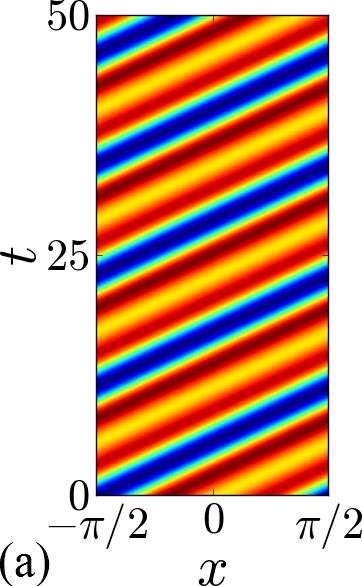
\includegraphics[width=0.22\textwidth]{2modes-conf-reqv}%
(b)\!\!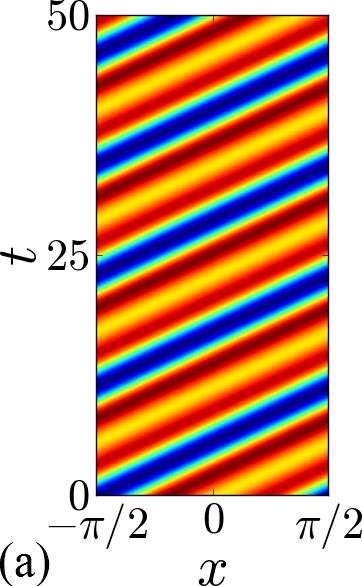
\includegraphics[width=0.22\textwidth]{2modes-conf-reqv}%
\caption{(Color online)
The \reqv\ \REQV{}{} in
 (a) the full \statesp, becomes an \eqv\ in
 (b) the symmetry-reduced configuration space.
}
\label{fig:2modes-conf-reqv}
\end{figure}

\begin{figure}%[H]
\centering
(a)\!\!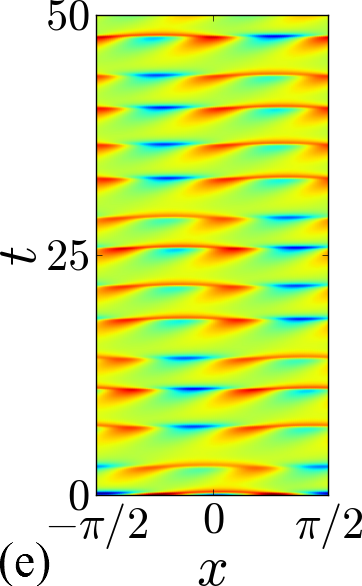
\includegraphics[width=0.22\textwidth]{2modes-conf-ergodic}
(b)\!\!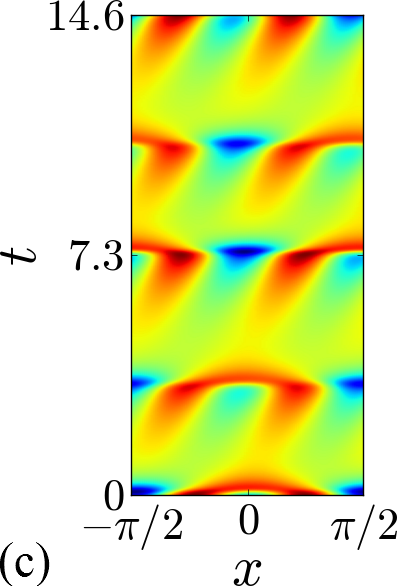
\includegraphics[width=0.22\textwidth]{2modes-conf-rpo}%
\caption{(Color online)
 (a) A typical ergodic trajectory of the \twomode\ system in the
 symmetry-reduced configuration space; clearly the unstable \reqv\
 \REQV{}{} in \reffig{fig:2modes-conf-reqv}\,(b) is far from a typical
 state.
 (b) Two repeats of \rpo\ \cycle{01}  (note the different time scale),
 in the symmetry-reduced configuration space. The dynamics is mostly
 dominated by the $m=1$ Fourier mode, interspersed by rapid shifts by
 $\approx \pm L/2$, dominated by the  $m=2$ Fourier mode.
}
\label{fig:2modes-conf}
\end{figure}

\begin{figure}%[H]
\centering
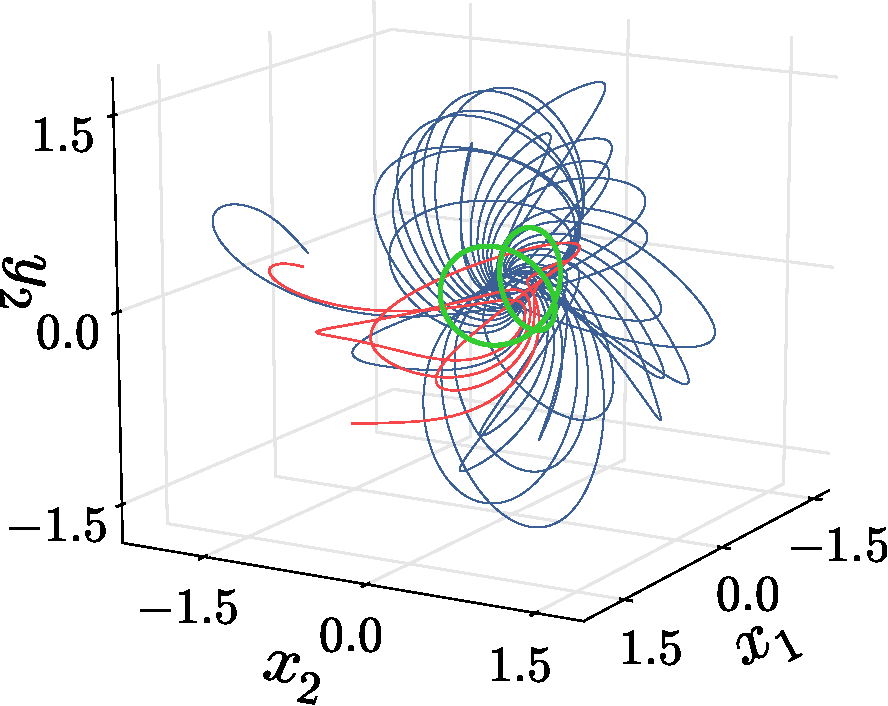
\includegraphics[width=0.45\textwidth]{2modes-ssp}
\caption{(Color online)
The same trajectories as in \reffig{fig:2modes-conf},
colored green, red and blue respectively,
in a 3D projection of the 4\dmn\ \statesp.
}
\label{fig:2modes-ssp}
\end{figure}

\begin{figure}%[H]
\centering
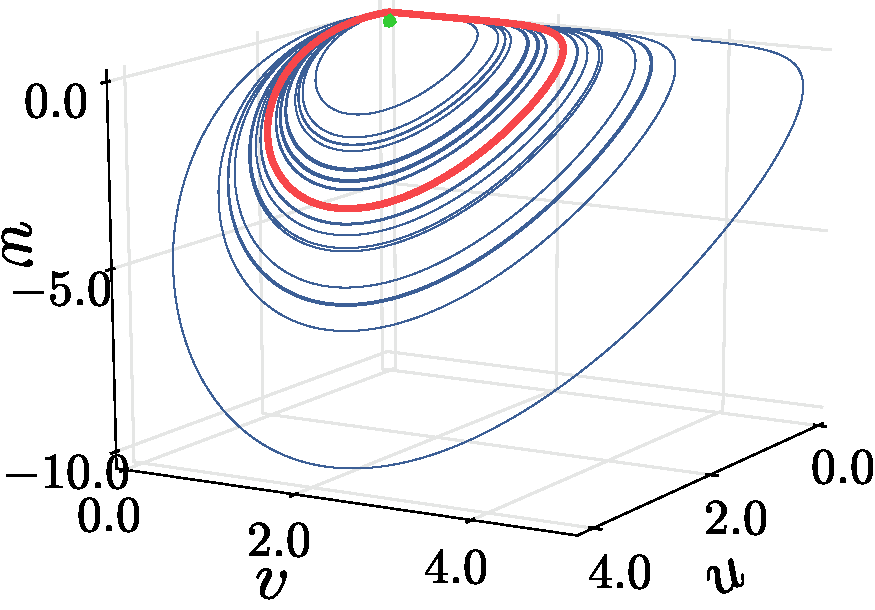
\includegraphics[width=0.45\textwidth]{2modes-invpol}
\caption{(Color online)
The same trajectories as in \reffig{fig:2modes-conf} and
\reffig{fig:2modes-conf-reqv}\,(a), colored green, red
and blue respectively, in a terms of 3 invariant polynomials.
The \reqv\ \REQV{}{} is now reduced to an \eqv, the green point.
}
\label{fig:2modes-invpol}
\end{figure}

\begin{figure}%[H]
\centering
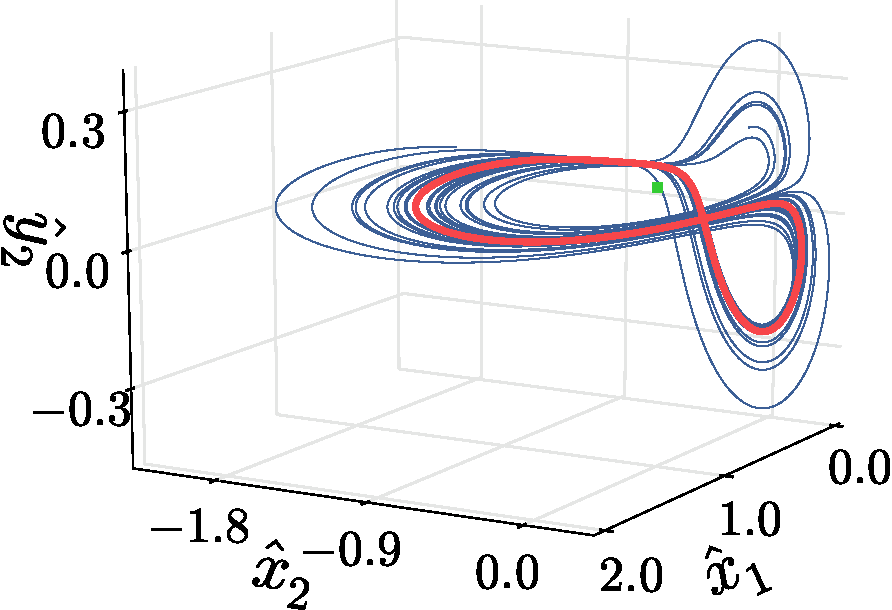
\includegraphics[width=0.45\textwidth]{2modes-sspRed}
\caption{(Color online)
The same trajectories as in \reffig{fig:2modes-conf} and
\reffig{fig:2modes-conf-reqv}\,(a), colored green, red
and blue respectively, in the 3\dmn\  first Fourier mode \slicePlane. The
\reqv\ \REQV{}{} is now reduced to an \eqv, the green point. In contrast
to the invariant polynomial representation \reffig{fig:2modes-invpol},
the qualitative difference between shifts by $\approx L/2$ and $\approx
-L/2$ in near passages to the {\sliceBord} is very clear, and it leads to
the unimodal Poincar\'e return map of \reffig{fig:psectandretmap}.
}
\label{2modes-sspRed}
\end{figure}

\PC{2014-07-14
Why $\pm L/2$ in \reffig{fig:2modes-conf} and
\reffig{fig:2modes-conf-reqv} and not $\pm \pi$?
}
\ES{2014-05-15}{I have replaced the second-mode slice, double-angled
figure in \reffig{2modes-conf-reqv}\,(b) with one resulting by integrating on the
$(0,0,1,0)$ slice, for consistency with panel (c). I hope Burak will
replace it with a publication quality figure of the same representation.
The trick of angle doubling will be introduced in its own section. }

To illustrate the \mslices\ on the \twomode\ system we choose a simple
set of parameters for which we observe interesting dynamics. These
parameters are listed in \refeq{eq:pars}. With this set of parameters,
we can write \twomode\ ODEs \refeq{eq:DangSO2} in terms of three parameters
$\{ \mu_1, c_2, a_2 \}$:
\bea
\label{eq:DangSO2set1}
  \sspC_1 &=& \mu_1 \,z_1 - z_1|z_1|^2 +c_1\,\overline{z}_1\,z_2
  \continue
  \sspC_1 &=& (1-\ii)\,{z_2}+a_2\,z_2|z_1|^2+\,z_1^2
\,,
\eea
Note that by setting $b_2 = 0$, we send the \reqv\ at $\invpol =
(0,-\mu_2/b_2,0,0)$ to infinity. Moreover, \refeq{PKinvEqs5a} yields
$\tilde{v} = (\mu_1 + \tilde{a}_1 \tilde{u})/(\mu_2 + \tilde{a}_2
\tilde{u} - \tilde{u} \tilde{b}_1)$. Substitution into \refeq{PKinvEqs5b}
allows one to solve for a single variable. By solving \refeq{PKinvEqs5}
with the parameter set \refeq{eq:pars}, we get two real roots, with
non-negative $u$ and $v$:
%the \eqva\ of the system in the invariant polynomial basis \refeq{Dang86(1.2)PK} as
\[
	\invpol_{\EQV{}} = (0,0,0,0)^T %\qquad \mbox{(double)}
\]
which is a double root and corresponds to an equilibrium of \refeq{eq:DangSO2}, and
\[
			 \invpol_{\REQV{}{}} = (0.193569,0.154131,-0.149539,-0.027178)^T\,,
\]
which is a {\reqv}. In real representation, a
representative point on  \REQV{}{} may be chosen as
\[
  \left(x_1, y_1, x_2, y_2\right) = \left(0.439966, 0, -0.386267, 0.070204\right)
\]
We visualize the dynamics of the \twomode\ system in four different
representations: 3D projections of the four-dimensional real valued
\statesp\ and invariant polynomials, in the 3D \slicePlane\ and on the 2D
configuration space plots on which the color-coded field $u(\conf,\zeit)$
is defined as follows:
\bea
	u(\conf, \tau) &=& \sum_{k=-2}^{2} \sspC_k(\zeit) e^{i k \conf}\, ,
	\continue && \mbox{where} \, \sspC_{-k} = \sspC_k^* \, \mbox{and} \,
	\sspC_0 = 0
\, .
\eea
\refFig{fig:2modes-conf}, \reffig{fig:2modes-conf-reqv}\,(a)
and \reffig{2modes-sspRed} show the sole \reqv\
\REQV{}{}, the \rpo\ \cycle{01}, and an ergodic trajectory of the
\twomode\ system in the four different representations discussed above.
Note that translation of the \reqv\ in the configuration space
\reffig{fig:2modes-conf-reqv}\,(a), corresponds to the \SOn{2} rotations in
the \statesp\ of Fourier modes in \reffig{2modes-ssp} (green curve) and
these orbits correspond to a single point in the symmetry reduced
representations of \reffig{fig:2modes-invpol} and \reffig{2modes-sspRed}.
Note also that the \rpo\ \cycle{01} translates/rotates as it advances in
configuration space (\reffig{fig:2modes-conf}\,(b)) and in the
equivariant \statesp\ \reffig{2modes-sspRed} (\reffig{2modes-ssp}),
whereas in the symmetry reduced plots (\reffig{fig:2modes-invpol} and
\reffig{2modes-sspRed}), it closes onto itself after one period.

\subsection{Finding cycles}

The simple structure of the symmetry reduced dynamics allows us to
determine the \rpo s of the \twomode\ system by means of a Poincar\'e
section and a return map. We illustrated this procedure in
\reffig{fig:psectandretmap}. Starting with an initial point close to the
\REQV{}{}, we computed a long ergodic trajectory of the symmetry reduced
\twomode\ system by integrating \refeq{e-so2red1stmode} (blue curve in
\reffig{fig:psectandretmap}\,{a)) and recorded its intersections (marked
with red in \reffig{fig:psectandretmap}\,{a)) with the Poincar\'e section
(transparent plane in \reffig{fig:psectandretmap}\,{a)), which includes
the \REQV{}{} and the imaginary part of its unstable stability
eigenvector (one of the green arrows in \reffig{fig:psectandretmap}\,{a)).
We then projected these intersections onto a basis $(v_1, v_2)$, which
spans the Poincar\'e section, and fit cubic splines to this set of
points, see \reffig{fig:psectandretmap}\,{b). The return map of arclengths
from the origin which is set to \REQV{}{} in
\reffig{fig:psectandretmap}\,{b), is unimodal with an sharp cusp located at its critical point, shown
in \reffig{fig:psectandretmap}\,{c). Note that the region corresponds to
the neighborhood of the \reqv\ $s = (0, 0.6)$ is never visited once the
flow leaves it and falls onto the chaotic attractor. For this reason, we
re-drew this return map after discarding the data corresponding to the
initial transients in \reffig{fig:psectandretmap}\,{d). We use this return
map to determine the accessible \rpo s  with their respective binary
symbol sequences.

\begin{figure}
\centering
  (a) 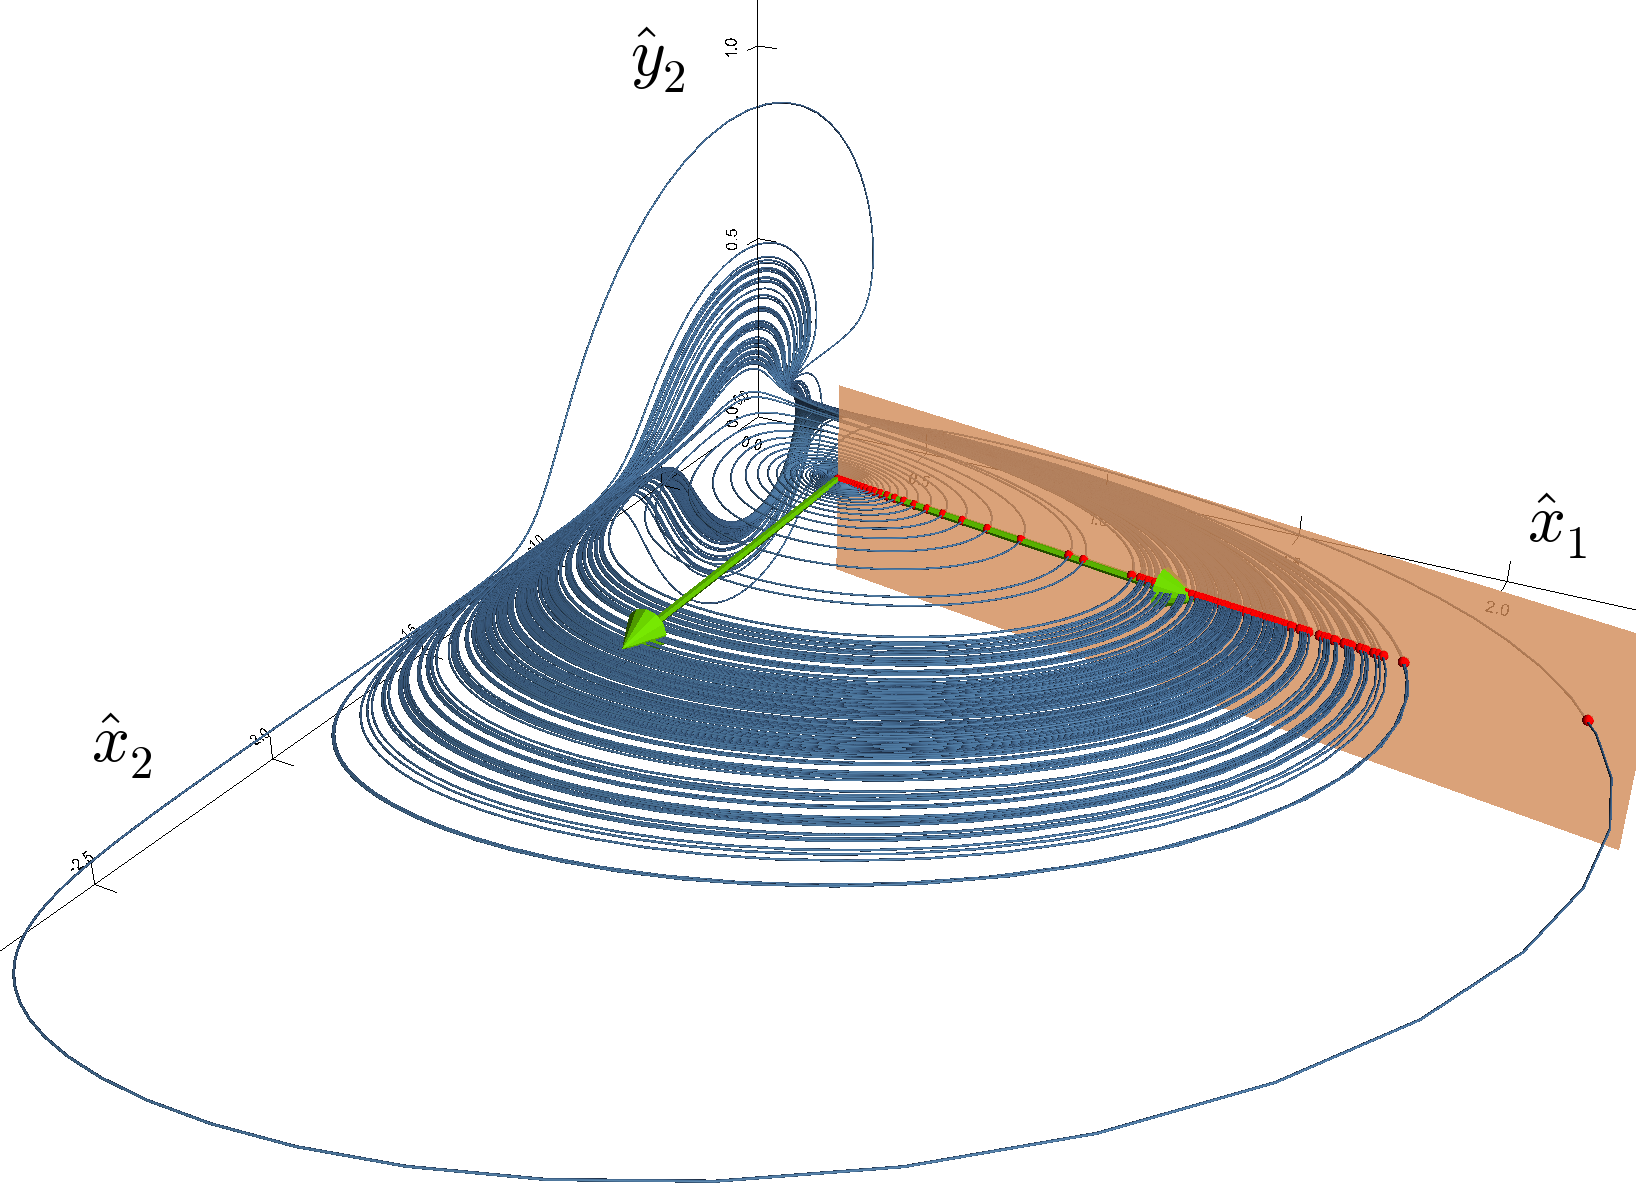
\includegraphics[width=0.45\textwidth]{BBpsecthd} \\
  (b) 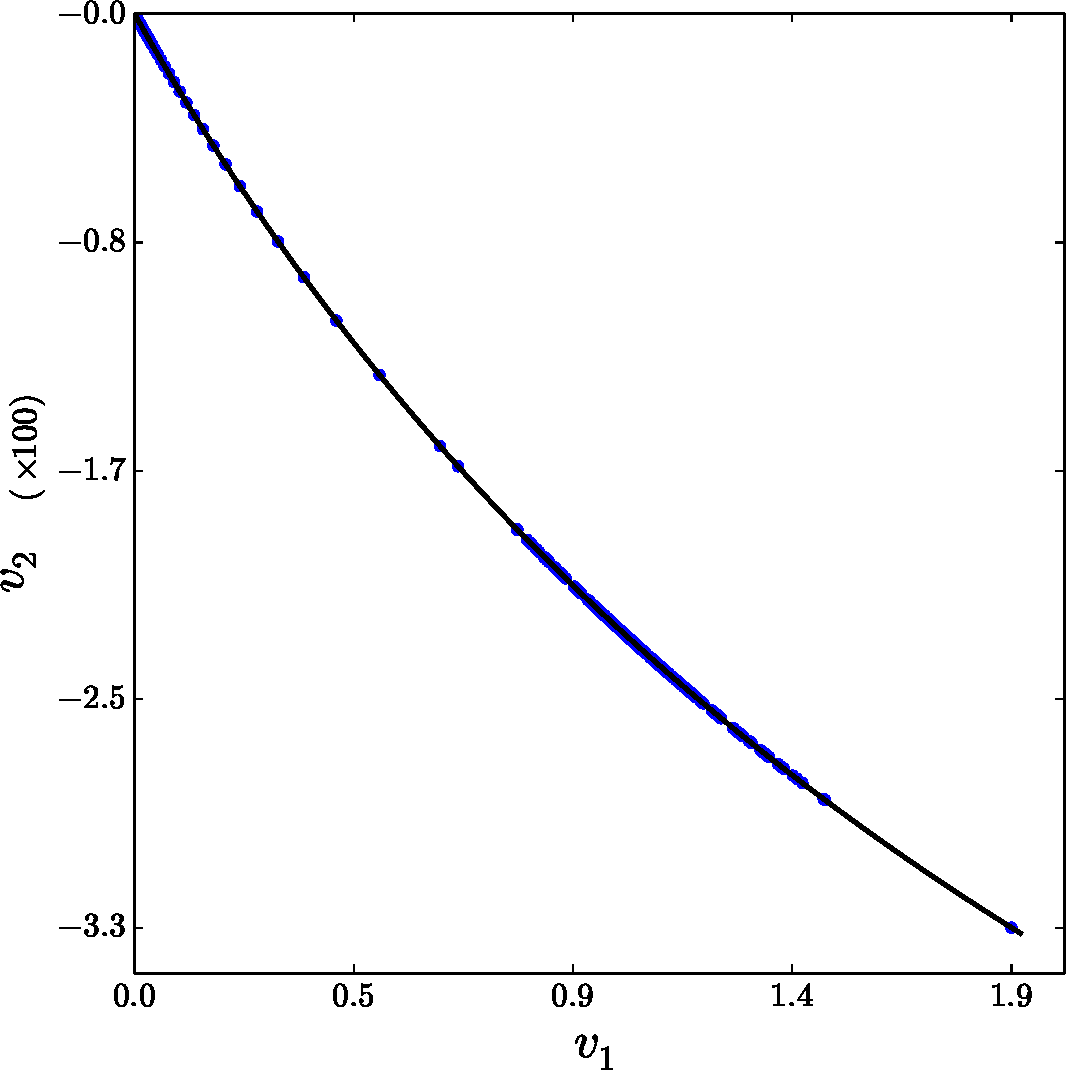
\includegraphics[width=0.20\textwidth]{BBpsectonslice}
  (c) 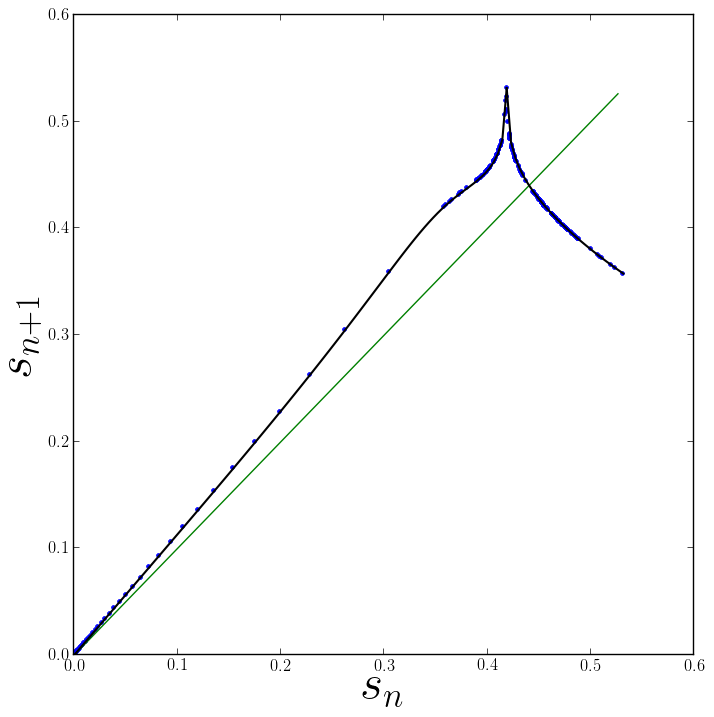
\includegraphics[width=0.20\textwidth]{BBretmaponslice} \\
  (d) 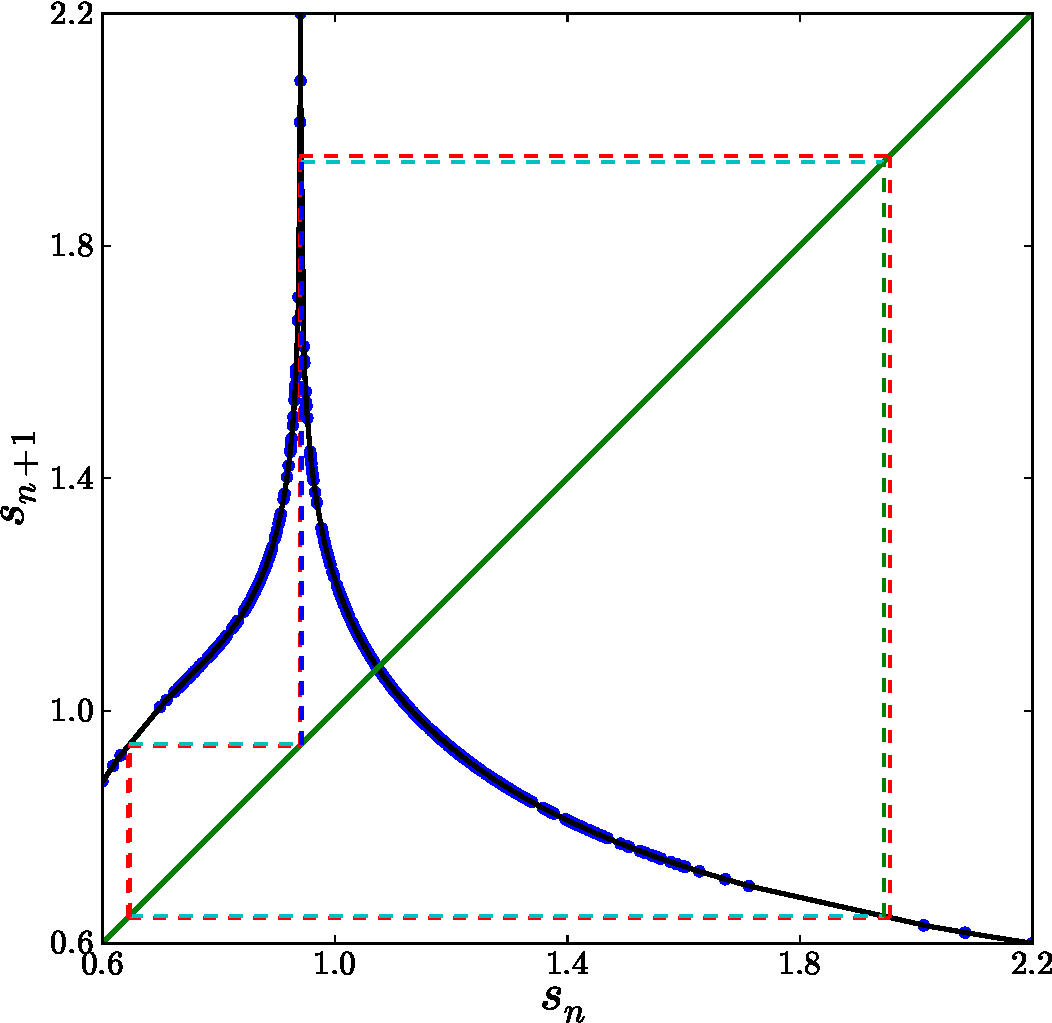
\includegraphics[width=0.45\textwidth]{BBretmaponsliceZoom}
\caption{(a) Symmetry reduced flow within the slice hyperplane (blue).
			Green arrows show the real and imaginary part of the unstable stability
			eigenvector $v_u$ of \REQV{}{}. A Poincar\'e section which includes
			$Im[v_u]$ is visualized as a transparent plane, and sections
			of the flow by the Poincar\'e section are marked with red.
		 (b) The Poincar\'e section which includes the \REQV{}{} and $v_u$ projected
			on to the basis within the plane shown in (a). Included is a
            transient trajectory initiated close to \REQV{}{}. Note that
		  	the vertical axis is magnified by $100$.
		 (c) The Poincar\'e arclength return map for the
		    Poincar\'e section (b).
		 (d) The return map without the transient points, framed by
            orbit of the critical point.
		 	Dashed lines show the 3-cycles \cycle{001} (red) and \cycle{011} (cyan).}
\label{fig:psectandretmap}
\end{figure}

Unimodal return map of \reffig{fig:psectandretmap}\,(d) lets us name the
periodic orbits of the \twomode\ system according to their binary
symbolic dynamics. Critical point of this map is at $s_C=0.98102264$,
corresponding to the tip of the return map. Topological coordinate of the
critical point, the kneading value, lets us determine the all admissible
cycles of the system. For a detailed introduction to the symbolic
dyanmics techniques we refer to \refref{DasBuch}. After determining the
admissible cycles, we find candidates corresponding to the admissible
symbol sequences from the return map, and feed them into a multiple
shooting Newton solver (see Appendix \ref{s:newton}) to precisely
determine the \rpo s. This way, we found the admissible cycles of the
\twomode\ system upto the topological length 12. In
\reffig{f-2modesrpofirst4} we show shortest $4$ of the \rpo s of the
\twomode\ system within the first Fourier mode \slicePlane . As seen from
\reffig{f-2modesrpofirst4}, trajectories of \cycle{001} and \cycle{011}
almost overlap in a large region of the \statesp . This behavior is also
manifested in the return map of \reffig{fig:psectandretmap}\,{d), where
we have shown cycles \cycle{001} and \cycle{011} with red and cyan
respectively. This is a general property of the \twomode\ cycles with odd
topological lengths: They come in pairs with almost equal Floquet
exponents, see \reffig{f-2modes-lambdaDist}.

\begin{figure}%[H]
\centering
 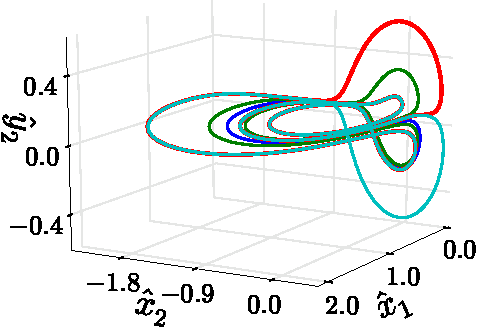
\includegraphics[width=0.45\textwidth]{2modesrpofirst4}
\caption{Shortest four \rpo s of the \twomode\ system: \cycle{1} (dark blue), \cycle{01} (green), \cycle{001} (red), \cycle{011} (cyan). Note that \rpo s \cycle{001} and \cycle{011} almost overlap everywhere except $\hat{x}_1 \approx 0$ .}
\label{f-2modesrpofirst4}
\end{figure}

\subsection{\CycForm s}
\label{s:DynAvers}

Spectrum of an observable, such as phase drift, or energy dissipation, of
a dynamical system is dual to the spectrum of its periodic orbits by
means of the classical trace formula\rf{DasBuch}
\beq
\sum_{\alpha=0}^{\infty} \frac{1}{s-s_{\alpha}} = \sum_p T_p \sum_{r=1}^{\infty} \frac{e^{r(\beta A_p - s T_p)}}{\oneMinJ{r}} .
\ee{e-ClassicalTraceFormula}

\begin{figure}%[H]
\centering
 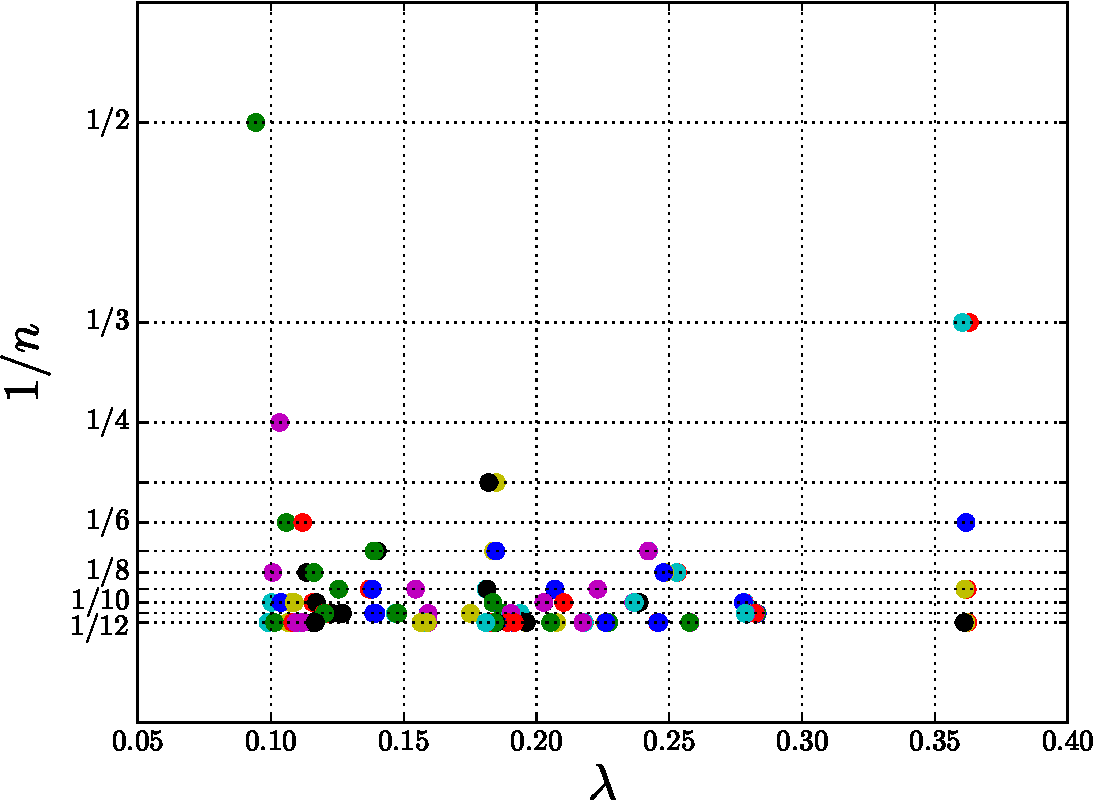
\includegraphics[width=0.45\textwidth]{2modes-lambdaDist}
\caption{Distribution of the leading Floquet exponents of \twomode\ cycles.}
\label{f-2modes-lambdaDist}
\end{figure}


Here, $s_{\alpha}$ are the eigenvalues of $\mathcal{A}$, the semigroup generator of the dynamical evolution of the observable $A$, outer sum on the RHS runs over the ``prime cycles'' of the system, $T_p$ is the period of the prime cycle $p$, $A_p$ is the value of the observable along the prime cycle, $\monodromy_p$ is the transverse (no marginal directions) monodromy matrix and $s$ and $\beta$ are auxilliary variables dual to the observable $A$ and time respectively.

While the classical trace formula \refeq{e-ClassicalTraceFormula} manifests the essential duality between the spectrum of an observable and that of the periodic orbits, in practice, it is hard to work with since the eigenvalues are located at the poles of
\refeq{e-ClassicalTraceFormula}. For this reason, one expresses this duality equivalently as the following spectral determinant
\beq
    \det (s-\mathcal{A}) = \exp \left( - \sum_p \sum_{r=1}^{\infty}
                             \frac{1}{r} \frac{e^{r(\beta A_p - s T_p)}}{\oneMinJ{r}} \right)\, ,
\ee{e-SpectralDeterminant}
logarithmic derivative of which gives \refeq{e-ClassicalTraceFormula}. The spectral determinant \refeq{e-SpectralDeterminant} is easier to work with since the spectrum of $\mathcal{A}$, is now located at the zeros of \refeq{e-SpectralDeterminant}. Convergence of \refeq{e-SpectralDeterminant} is still not obvious. More insight is gained by approximating $\oneMinJ{r}$ by the product of expanding Floquet multipliers and then computing the $r$ sum in \refeq{e-SpectralDeterminant}.
\bea
\oneMinJ{} &=& | (1 - \ExpaEig_{e,1})(1 - \ExpaEig_{e,2})... \continue
			&&(1 - \ExpaEig_{c,1}) (1 - \ExpaEig_{c,2}) ... | \nonumber \\
			&\approx& \prod_e |\ExpaEig_e| = |\ExpaEig_p|,
\eea
where $|\ExpaEig_{e,i}| > 1$ and $|\ExpaEig_{c,i}| < 1$ are expanding and contracting Floquet multipliers respectively. After this approximation, $r$-sum in \refeq{e-SpectralDeterminant} becomes the Taylor expansion of natural logarithm and it can be compactly written as follows:
\beq
1 / \zeta = \prod_r (1 - t_p) \, \mbox{where}, \, t_p = \frac{1}{|\ExpaEig_p|} e^{\beta A_p - s T_p} z^{n_p} .
\ee{e-DynamicalZeta}
Where we inserted the `order tracking' term $z$. For complete binary symbolic dynamics, the dynamical zeta function \refeq{e-DynamicalZeta} can be brought into the `curvature expansion' form:
\bea
1 / \zeta &=& 1 - t_0 - t_1 - (t_{01} - t_0 t_1 )  \label{e-CycleExpansion} \\
		  && - [(t_{011} - t_{01}t_1) + (t_{001} - t_{01} t_0)] - ... \continue
		  &=& 1 - \sum_f t_f - \sum_n \hat{c}_n \label{e-CurvatureExpansion}.
\eea
In the curvature expansion \refeq{e-CurvatureExpansion}, we grouped the contributions to the dynamical zeta function as `fundamental' contributions $t_f$ and `curvature' corrections. One expects the curvature corrections to be small since the longer prime cycles are `shadowed' by the combination of the shorter ones, the `pseudocycles'.

For complete binary symbolic dynamics, the only fundamental contributions to the dynamical zeta function are the cycles with topological length $1$, see \refeq{e-CurvatureExpansion}. This is not the case for any map since in general there might be non-trivial pruning rules, hence longer cycles can appear unshadowed. The Poincar\'e return map of \reffig{fig:psectandretmap}\,{d) is such a map with non-trivial pruning rules, however, note that cycles \cycle{001} and \cycle{011} passes very close to the tip of the cusp, the critical point, in \reffig{fig:psectandretmap}\,{d). This observation motivates us to approximate the return map of \reffig{fig:psectandretmap}\,{d), as if its tip is located at $s = 0.97986453$, where the cycle \cycle{001} lands, and omit the contributions above this point. We will refer this approximation as the `finite grammar approximation' since by doing it, we obtain single pruning rule; that is the symbol sequence $00$ is not allowed. This grammar is known as the `golden mean' pruning and a complete binary symbolic dynamics can be converted to the golden mean symbolic dynamics by substitution $0 \rightarrow 01$. We can write the dynamical zeta function for the golden mean pruned symbolic dynamics by replacing $0$s in \refeq{e-CycleExpansion} by $01$:
\bea
1 / \zeta &=& 1 - t_{01} - t_1 - (t_{011} - t_{01} t_1 ) \label{e-GoldenMeanCycleExpansion}\\
		  && - [(t_{0111} - t_{011}t_1) + (t_{01011} - t_{01} t_{011} ) ] - ... \nonumber
\eea
Note that all the contributions longer than topological length $2$ to the golden mean dynamical zeta function are in form of shadowing combinations. However, as we shall see, they are not small.

While dynamical zeta functions are useful for investigating the convergence properties, they are not exact, and their computational cost is same with that of the exact spectral determinants. For this reason, we will expand the spectral determinant \refeq{e-SpectralDeterminant} ordered in the topological length of cycles and pseudocycles as follows:
\beq
    \det (s-\mathcal{A}) =   \prod_p \exp \left( - \sum_{r=1}^{n_p r < N}
                             \frac{1}{r} \frac{e^{r(\beta A_p - s T_p)}
                                          }{\oneMinJ{r}} z^{n_p r} \right) \, .
\ee{e-SpectralDeterminantExp}
This is the form that we use to compute the spectral determinant. For each prime cycle, we compute the sum term in \refeq{e-SpectralDeterminantExp} truncated at the expansion order $N$, and then expand the exponential upto order $N$, and multiply this expansion with the contributions from previous cycles and drop terms with order greater than $N$. This way, we obtain the $N^{th}$ order spectral determinant \refeq{e-SpectralDeterminant}. Let us denote the resultant series after setting $z=1$ as
\beq
    F_N(s, \beta ) = 1 - \sum_{n=1}^{N} Q_n(s, \beta ) \, .
    \label{e-NthOrderSpectDet}
\eeq
Leading $0$ of $F_N(s, 0)$, $s_0$, corresponds to the leading eigenvalue of the Perron-Forbenius operator, $\gamma_0 = - s_0$, which can be interpreted as the `escape rate'. We expect the escape rate to be small, ideally zero, if the cycle expansion is good.
After finding $s_0$, we can compute the dynamical averages as follows:
Mean period:
\bea
    \langle T \rangle_N &=& \left. \frac{\partial F_N}{\partial s}
                            \right|_{\beta=0, s=s_0} \, , \label{e-AveragePeriod} \\
    \langle A \rangle_N &=& - \left.
                              \frac{\partial F_N}{\partial \beta}
                              \right|_{\beta=0, s=s_0} \, ,   \label{e-AvgA} \\
    \langle (A - \langle A \rangle )^2 \rangle_N
    &=& - \left. \frac{\partial^2 F_N}{\partial \beta^2} \right|_{\beta=0,
                                                  s=s_0} \, , \label{e-AvgSigma} \\
    \langle a \rangle_N &=& - \frac{1}{\langle T \rangle_N} \left.
                              \frac{\partial F_N}{\partial \beta}
                              \right|_{\beta=0, s=s_0} \, ,   \label{e-Avga} \\
    \langle (a - \langle a \rangle )^2 \rangle_N
    &=& - \frac{1}{\langle T \rangle_N} \left. \frac{\partial^2 F_N}{\partial \beta^2} \right|_{\beta=0,
                                                                    s=s_0} \, \label{e-Avgsigma} .
\eea
Here, $\langle T \rangle_N$ is average cycle period, $A$ denotes an observable that is ``additive'' along the trajectories, in other words, that satisfies semi-group property; and $a$ a is the rate of that observable. For example, for $A = \phi$, \refeq{e-AvgA} yields the ``average phase shift per cycle'', whereas \refeq{e-Avga} yields ``average phase speed''. Variances \refeq{e-AvgSigma} and \refeq{e-Avgsigma} are respectively interpreted similarly as the ``variance per cycle'' and ``variance rate'' of an observable.

We computed escape rate $\gamma$, average cycle period $\langle T \rangle$, leading Lyapunov exponent $\Lyap$, average phase speed $\langle \dot{\phi} \rangle$ and the phase diffusion constant $D$ of the \twomode\ system using cycle averaging formulas \refeqs{e-AveragePeriod}{e-Avgsigma}. We listed our findings with respect to the increasing expansion order in \reftab{t-DynamicalAverages} and \reftab{t-DynamicalAveragesNoGrammar}. While in \reftab{t-DynamicalAverages} we used the finite grammar approximation, in \reftab{t-DynamicalAveragesNoGrammar} we input all the cycles we found to the calculation.

\begin{table}
	\begin{tabular}{c|c|c|c|c|c}
	 $N$ & $\gamma$ & $\langle T \rangle$ & $\lambda$ & $\langle \dot{\phi} \rangle$ & $D$ \\ 
	\hline
	1 & 0.24983007 & 3.64151210 & 0.10834935 & 0.02223518 & 0.00090019 \\ 
 	2 & -0.01159743 & 5.89675999 & 0.10302904 & -0.14242535 & 0.22615040 \\ 
 	3 & 0.02744646 & 4.72713874 & 0.11849781 & -0.14916163 & 0.22541882 \\ 
 	4 & -0.00445545 & 6.23866097 & 0.10631075 & -0.22271184 & 0.54199883 \\ 
 	5 & 0.00068106 & 5.89674866 & 0.11842709 & -0.19506985 & 0.47091930 \\ 
 	6 & 0.00068491 & 5.89688492 & 0.11820055 & -0.21660997 & 0.64918118 \\ 
 	7 & 0.00063044 & 5.90316812 & 0.11835165 & -0.18083296 & 0.51935080 \\ 
 	8 & 0.00071488 & 5.89189180 & 0.11827587 & -0.21129228 & 0.78673581 \\ 
 	9 & 0.00072867 & 5.88975993 & 0.11826879 & -0.19203222 & 0.70977900 \\ 
 	10 & 0.00072808 & 5.88986409 & 0.11826793 & -0.20302879 & 0.90493496 \\ 
 	11 & 0.00072790 & 5.88989901 & 0.11826783 & -0.19453187 & 0.86683629 \\ 
 	\end{tabular}
	\caption{Cyle expansion estimates of the escape rate $\gamma$, average cycle period $\langle T \rangle$, Lyapunov exponent $\lambda$, average phase velocity $\langle \dot{\phi} \rangle$ and the diffusion coefficient $D$ with respect to the expansion order $N$ .}
	\label{t-DynamicalAverages}
\end{table}
\begin{table}
	\begin{tabular}{c|c|c|c|c|c}
	 $N$ & $\gamma$ & $\langle T \rangle$ & $\lambda$ & $\langle \dot{\phi} \rangle$ & $D$ \\ 
	\hline
	1 & 0.24982996 & 3.64151221 & 0.10834917 & 0.02223518 & 0.00090019 \\ 
 	2 & -0.01159761 & 5.89676053 & 0.10302891 & -0.14242516 & 0.22615014 \\ 
 	3 & 0.02261469 & 4.88995874 & 0.13055574 & -0.16698925 & 0.28645997 \\ 
 	4 & -0.00606560 & 6.24822611 & 0.11086469 & -0.22623282 & 0.55402655 \\ 
 	5 & 0.00091264 & 5.77716415 & 0.11812034 & -0.19839015 & 0.47840111 \\ 
 	6 & 0.00026210 & 5.83645342 & 0.11948918 & -0.21788301 & 0.65393430 \\ 
 	7 & 0.00001771 & 5.86382098 & 0.12058951 & -0.18565119 & 0.55022944 \\ 
 	8 & 0.00011328 & 5.85110445 & 0.12028459 & -0.21480977 & 0.80768111 \\ 
 	9 & 0.00017071 & 5.84222727 & 0.12010579 & -0.19376222 & 0.72685211 \\ 
 	10 & 0.00015683 & 5.84466944 & 0.12014022 & -0.20501316 & 0.92174228 \\ 
 	\end{tabular}
	\caption{Cyle expansion estimates of the escape rate $\gamma$, average cycle period $\langle T \rangle$, Lyapunov exponent $\lambda$, average phase velocity $\langle \dot{\phi} \rangle$ and the diffusion coefficient $D$ with respect to the expansion order $N$ .}
	\label{t-DynamicalAveragesNoGrammar}
\end{table}


We motivated our finite grammar approximation by expecting a fast convergence after second order in the cycle expansion, however,
this is not the case. The reason is, as we mentioned before, that the curvature corrections of \refeq{e-GoldenMeanCycleExpansion} are not small. This is due to the fact that the Floquet exponent of the cycle \cycle{011} (marked cyan at $1/3$ line of \reffig{f-2modes-lambdaDist}), is much larger than the rest of the set that appears in the cycle expansion, and since the cycle contributions are weighted by the inverse Floquet multipliers, $t_{011}$ almost cancels every shadowing combination it appears. Hence the curvature corrections in which $t_{011}$ appears as a shadowing orbit, are not small. However, we still get a better convergence comparing to the case where we include all cycles in the calculation. \refTab{t-DynamicalAverages} and \reftab{t-DynamicalAveragesNoGrammar} show that when the expansion order is $10$, the Lyapunov exponents converges with a $6$ digits in the finite grammmar calculations, whereas it has $4$ digit convergence in the case where we included all cycle contributions.

In order to compare with the cycle averages, we numerically estimated the
leading Lyapunov exponent of the \twomode\ system using the method of
Wolf \etal\rf{WolfSwift85}. This procedure was repeated 100 times for
different initial conditions, yielding a mean estimate of
$\Lyap_{Numerical} = 0.1198 \pm 0.0008$. While the finite grammar
estimate $\Lyap_{FG} = 0.118268$ is within $1\%$ range of this value,
the full cycle expansion agrees with the numerical estimate. This is not
surprising, since in the finite grammar approximation, we discard the
most unstable cycles, thus, we obtain a slightly smaller Lyapunov
exponent while obtaining a better convergence.

%\section{Cycle Averages}
\label{s:DynAvers}

So far, we have explained how we find the \rpo s of the \twomode\ system in
its \reducedsp\ and how to compute their stability. However, we have not yet
said anything about what to do with these numbers. We begin this section with
an overview of the main results of the periodic orbit theory, referring the reader
to \refref{DasBuch} for a detailed introduction to the subject. Our discussion
closely follows the presentation of \refref{DasBuch} with the addition of how
the theory is modified in the presence of continuous symmetries in
\refsect{s-ContFac}. In \refsect{s-CycExp}, we present cycle expansions and
explain how to approximate the Poincar\'e section in
\reffig{fig:psectandretmap} (d), in order to obtain a better convergence of
the spectral determinants. We finish this section with the numerical results in
\refsect{s-NumResults}

\subsection{Classical trace formula}
Consider the {\evOper}, the action of which evolves a density
$\rho_0(\ssp)$ in the \statesp :
\bea
    \rho(\zeit ,\ssp) &=& [\Lop^\zeit \rho_0 ] (\ssp) \, , \continue
    &=& \int d \ssp' \delta (\ssp - \flow{\zeit}{\ssp'})
        e^{\beta \Obser^\zeit (\ssp' )} \rho_0(\ssp') \, .
        \label{e-EvOper}
\eea
Here, $\beta$ is an auxiliary variable and $\Obser^\zeit (\ssp')$ is the
integrated value of an `additive' observable $\obser$ along the orbit
$\flow{\zeit}{\ssp'}$:
\beq
    \Obser^\zeit (\ssp' ) = \int_0^{\zeit} d \zeit'
                              \obser(\flow{\zeit'}{\ssp'}) \, .
\eeq
Notice that when $\beta = 0$, the \evOper\ \refeq{e-EvOper} simply evolves
the density of \statesp\ points to its new form after time $\zeit$. As we
shall see, attaching\DB{2014-11-3}{What does ``attaching'' mean in this context... might be lacking technical rigor here.}
the integrated observables to this operator enables us to
study values of these observables averaged over the invariant measures.

Since we required our observable to be additive along an orbit and
exponentiated its integrated value in the construction of the \evOper\
\refeq{e-EvOper}; the evolution operator itself is multiplicative:
\beq
    \Lop^{\zeit_1 + \zeit_2} = \Lop^{\zeit_2} \Lop^{\zeit_1} \, .
    \label{eq-SemiGroup}
\eeq
For the kernel of the evolution integral, which we will refer to as
$\Lop^\zeit (\ssp, \ssp')$ with explicit arguments, we can write this relation
as:
\beq
	\Lop^{\zeit_1 + \zeit_2} (\ssp,\ssp') =
    \int d\ssp'' \Lop^{\zeit_2} (\ssp, \ssp'')
                   \Lop^{\zeit_1} (\ssp'', \ssp) \, .
	\label{eq-SemiGroupKernel}
\eeq
This `semigroup property' \refeq{eq-SemiGroup} of the {\evOper} allows us to
define the {\evOper} as the formal exponential of its infinitesimal generator
\Aop :
\beq
	\Lop^t = e^{\Aop t} \, .
	\label{eq-EvOpExp}
\eeq
By definition \refeq{e-EvOper}, the eigenvalues and eigenfunctions of $\Lop^t$ (and
thus \Aop ) are functions of $\beta$. Let us define $\rho_{\beta} (x)$ as the
eigenfunction of \refeq{e-EvOper} corresponding to the leading eigenvalue (i.e., the one with the
largest real part); we can write the action of \refeq{e-EvOper} on this density
explicitly as follows:
\beq
    \left[ \Lop^t \rho_{\beta} \right] (x) = e^{t s(\beta )} \rho_{\beta} (x)
    \, .
    \label{eq-EigenvalueRel}
\eeq
Here, $s(\beta)$ is the eigenvalue of $\Aop$. As stated earlier, when
$\beta = 0$, the {\evOper} simply evolves densities; this form of the evolution
operator is known as the {\FPoper}. If we assume that the system under study is ergodic,
then an `invariant measure' $\rho_0(\ssp)$ exists with eigenvalue
$s(0) = 0$ exists. The long time spectrum of any observable is going to be dominated by
its average over such a density, hence we define the average of an observable
as its average over the invariant measure:
\beq
    \langle \obser \rangle = \int d \ssp \, \obser(\ssp) \rho_0 (\ssp) \, .
    \label{e-obserAvg}
\eeq
By evaluating the action of the {\evOper} \refeq{e-EvOper} for infinitesimal
times and after some algebra, which we skip here, one finds that the
averages of observables, as well as their higher moments, can be generated from the
derivatives of $s(\beta)$:
\beq
    \langle \obser \rangle =
        \left. \frac{d s}{d \beta} \right|_{\beta = 0} \, , \quad
    \langle (\obser - \langle \obser \rangle )^2 \rangle =
        \left. \frac{d^2 s}{d \beta^2} \right|_{\beta = 0} \,, ...
    \label{eq-moments}
\eeq
In order to obtain $s(\beta)$, we construct the resolvent of \Aop , by taking
the Laplace transform of \refeq{eq-EvOpExp}:
\beq
	\int_0^{\infty} d\zeit e^{-s\zeit} \Lop^\zeit = (s-\Aop)^{-1} \, ,
	\label{eq-ResolventA}
\eeq
the trace of which peaks at the eigenvalues of \Aop. By taking the
Laplace transform of $\Lop^\zeit$ and computing its trace
by $\tr \Lop^\zeit = \int d\ssp \Lop^\zeit (\ssp,\ssp)$, one obtains the
classical trace formula:
\beq
\sum_{\alpha=0}^{\infty} \frac{1}{s-s_{\alpha}} = \sum_p T_p
\sum_{r=1}^{\infty} \frac{e^{r(\beta \Obser_p - s T_p)}}{\oneMinJ{r}}
\ee{e-ClassicalTraceFormula}
that relates the spectrum of the {\evOper} to the spectrum of the periodic
orbits. Here,  $s$ is the auxiliary
variable of the Laplace transform and $s_{\alpha}$ are the eigenvalues of \Aop . The
outer sum on the right hand side runs over the `prime cycles' $p$ of the system,
which have periods $T_p$. $\Obser_p$ is the value of
the observable integrated along the prime cycle and $\monodromy_p$ is the transverse
monodromy matrix, the eigenvalues of which are the Floquet multipliers of $p$
excluding the marginal ones ($|\Lambda| \neq 1$). In the derivation of
\refeq{e-ClassicalTraceFormula}, one assumes that the flow has a single marginal direction,
namely the direction that is parallel to the periodic orbit at all times, and evaluates the
contribution of each \po\ to the trace integral by transforming to a local coordinate
system where one of the coordinates is
parallel to the flow while the rest is transverse. Integration along the
parallel direction is what contributes the factors of $T_p$. The transverse integral
over the delta function contributes the factor of $\oneMinJ{r}$.

\subsection{Continuous factorization}
\label{s-ContFac}

The classical trace formula \refeq{e-ClassicalTraceFormula} accounts for contributions from \po s
to long time dynamical averages. However, \rpo s of equivariant systems are almost never
periodic in the full \statesp. In order to compute the contributions of \rpo s
to the trace of the \evOper, one has to factorize
\DB{}{factor or factorize... not sure which sounds better...
are they different?}
the \evOper\
into the irreducible subspaces of the symmetry group. For discrete symmetries,
this procedure is studied in \refref{CvitaEckardt} and for the quantum systems
with continuous symmetries (Abelian and 3D rotations), factorization of
semiclassical Green's operator is carried out in \refref{Creagh93}.
\refRef{Cvi07} addresses the continuous factorization of the \evOper\ and its
trace; we provide a sketch of this treatment here. We start by stating, without
proof, that a square-integrable field $\psi (\ssp)$ over a vector space can be
factorized into its projections over the irreducible subspaces of a group
$\Group$:
\beq
    \psi (\ssp) = \sum_m \mathbb{P}_m \psi (\ssp) \, ,
\eeq
where the sum runs over the irreducible representations of the $\Group$ and
the projection operator onto the $m$th irreducible subspace, for a continuous
group, is:
    \PC{2014-11-10: From now on, a problem - if I redefine $D(\cdots)$ as \matrixRep,
    cannot easily revert to the concise $g$ notation...}
\beq
    \mathbb{P}_m = d_m \int_\Group d \mu(\LieEl) \chi_m (\LieEl(\theta))
                            \mathbb{D}(\theta)
\,.
\ee{e-ProjectionOperator}
Here, $d_m$ is the dimension of the representation, $d \mu(g)$ is the
normalized `Haar measure', $\chi_m (\LieEl)$ is the `character' of $m$th
irreducible representation and $\mathbb{D}(\theta)$ is the operator which
transforms a scalar field defined on \statesp\ according to $\matrixRep(\theta)$,
namely, $\mathbb{D}(\theta) \rho (\ssp) = \rho(\LieEl^{-1}(\theta) \ssp)$.
    \DB{2014-11-3}{Added missing parenthesis to
    this expression. Did I put it in the right place? I think so, but please double check.}
For
our specific case of single $\SOn{2}$ symmetry,
\bea
d_m &\rightarrow& 1\, , \\
\int_G d \mu(g) &\rightarrow& \oint \frac{d \theta} {2 \pi} \, , \\
\chi_m (\LieEl(\theta)) &\rightarrow& e^{- \ii m \theta } \, .
\eea
Since the projection
operator \refeq{e-ProjectionOperator} factorizes scalar fields in the \statesp\
into their projections onto irreducible subspaces of the $\Group$, it can be used to
factorize the \evOper\ since the \evOper\ acts on scalar
fields (densities) and returns scalar fields on the \statesp . Thus the kernel
of the \evOper\ transforms under the action of $\mathbb{D}(\theta)$ as:
\bea
    \mathbb{D}(\theta) \Lop^t (\ssp', \ssp) &=&
        \Lop^t (\LieEl^{-1}(\theta) \ssp', \ssp)\,,
    \continue
    &=& \Lop^t (\ssp', \matrixRep(\theta) \ssp) \,, \continue
    &=& \delta (\ssp' - \matrixRep(\theta) f^t (\ssp)) e^{\beta \Obser^t(\ssp)}\, ,
    \label{e-gEvOper}
\eea
where the second step followed from the equivariance of the system under
consideration. \Rpo s contribute to the $\mathbb{P}_m \Lop^t = \Lop_m^t$ since when its
kernel is modified as in \refeq{e-gEvOper}, the projection involves an integral
over the group parameters that will be non-zero at the phase shift of the
\rpo s. By computing the trace of $\Lop_m^t$, which in addition to the integral
over \statesp , now involves another integral over the group parameters, one
obtains the $m$th irreducible subspace contribution to the classical trace as
\beq
\sum_{\alpha=0}^{\infty} \frac{1}{s-s_{m, \alpha}} = \sum_p T_p
\sum_{r=1}^{\infty} \frac{\chi_m (\LieEl^r(\theta_p))
            e^{r(\beta \Obser_p - s T_p)}}{\oneMinJred{r}} .
\ee{e-ReducedTraceFormula}
The reduced trace formula \refeq{e-ReducedTraceFormula} differs from the
classical trace formula \refeq{e-ClassicalTraceFormula} by the group character
term, which is evaluated at the \rpo\ phase shifts, and the reduced monodromy
matrix $\monodromyRed$, which is the $(d-N-1)\times(d-N-1)$ reduced Jacobian
for the \rpo\ evaluated on a Poincar\'e section in the \reducedsp . The eigenvalues
of $\monodromyRed$ are those of the \rpo\ Jacobian \refeq{e-rpoJacobian}
excluding the marginal ones, i.e., the ones corresponding to time evolution and evolution
along the continuous symmetry directions.

Since we are only interested in the leading eigenvalue of the \evOper , we are
going to consider contributions only from the $0$th irreducible subspace to the
trace \refeq{e-ClassicalTraceFormula} from its projections
\refeq{e-ReducedTraceFormula} which we can write for our $\SOn{2}$ case
explicitly as \DB{2014-11-3}{This sentence is weird but I'm kind of lost at this point, so
I don't know how to fix it.}
\beq
\sum_{\alpha=0}^{\infty} \frac{1}{s-s_{0, \alpha}} = \sum_p T_p
\sum_{r=1}^{\infty} \frac{e^{r(\beta \Obser_p - s T_p)}}{\oneMinJred{r}} \, .
\ee{e-tracem0}
This form differs from the classical trace formula
\refeq{e-ClassicalTraceFormula} only by the reduced monodromy matrix since
the $0$th irreducible representation of $\SOn{2}$ has character $1$. For this
reason, cycle expansions \rf{AACI}, which we will cover next, are applicable
to \refeq{e-tracem0} after the replacement
$\monodromy \rightarrow \monodromyRed$.

\subsection{Cycle expansions}
\label{s-CycExp}

While the classical trace formula \refeq{e-ClassicalTraceFormula} and its
factorization for systems with continuous symmetry \refeq{e-ReducedTraceFormula} manifest
the essential duality between the spectrum of an observable and that of
the \po s and \rpo s, in practice, they are hard to work with since the
eigenvalues are located at the poles of \refeq{e-ClassicalTraceFormula} and
\refeq{e-ReducedTraceFormula}. The dynamical zeta function
\refeq{e-DynamicalZeta}, which we derive below provides a perturbative expansion form,
which enables us to order terms in decreasing importance while computing
spectra for the \twomode\ system. As stated earlier, \refeq{e-tracem0}
is equivalent to the \refeq{e-ClassicalTraceFormula} via substitution
$\monodromy \rightarrow \monodromyRed$. We start by defining the
`spectral determinant':
\beq
  \det (s-\Aop) = \exp \left( - \sum_p \sum_{r=1}^{\infty}
      \frac{1}{r} \frac{e^{r(\beta \Obser_p - s T_p)}}{\oneMinJ{r}} \right)\, ,
\ee{e-SpectralDeterminant}
whose logarithmic derivative ($(d/ds) \ln \det(s - \Aop)$) gives
the classical trace formula \refeq{e-ClassicalTraceFormula}.
The spectral determinant \refeq{e-SpectralDeterminant} is easier to work
with since the spectrum of $\mathcal{A}$ is now located at the zeros of
\refeq{e-SpectralDeterminant}. The convergence of \refeq{e-SpectralDeterminant}
is, however, still not obvious. More insight is gained by approximating
$\oneMinJ{r}$ by the product of expanding Floquet multipliers and then
carrying out the sum over $r$ in \refeq{e-SpectralDeterminant}. This
approximation yields
\bea
\oneMinJ{} &=& | (1 - \ExpaEig_{e,1})(1 - \ExpaEig_{e,2})... \continue
			&&(1 - \ExpaEig_{c,1}) (1 - \ExpaEig_{c,2}) ... | \nonumber \\
			&\approx& \prod_e |\ExpaEig_e| \equiv |\ExpaEig_p|,
    \label{e-LambdapApprox}
\eea
where $|\ExpaEig_{e,i}| > 1$ and $|\ExpaEig_{c,i}| < 1$ are expanding and
contracting Floquet multipliers respectively. The sum over $r$ in
\refeq{e-SpectralDeterminant} becomes the Taylor expansion of natural logarithm
after approximation \refeq{e-LambdapApprox}. Carrying out this sum, brings the
spectral determinant \refeq{e-SpectralDeterminant} to a product (over prime
cycles) known as the dynamical zeta function:
\beq
1 / \zeta = \prod_p (1 - t_p) \, \mbox{where}, \, t_p = \frac{1}{|\ExpaEig_p|}
            e^{\beta \Obser_p - s T_p} z^{n_p} .
\ee{e-DynamicalZeta}
We multiplied each `cycle weight' $t_p$ by the `order tracking term' $z^{n_p}$
where $n_p$ is the topological length of the $p$th prime cycle. This polynomial
ordering arises naturally in the study of discrete time systems where the
Laplace transform is replaced by $z$-transform. Here, we insert the powers of
$z$ by hand and we will set its value to $1$ at the end of calculations. The
reason for doing this is to write the dynamical zeta function
\refeq{e-DynamicalZeta} in the `cycle expansion' form, after grouping its
terms in powers of $z$. For complete binary dynamics, where every binary symbol
sequence is accessible, the cycle expansion reads
\bea
1 / \zeta &=& 1 - t_0 - t_1 - (t_{01} - t_0 t_1 )  \label{e-CycleExpansion} \\
		  && - [(t_{011} - t_{01}t_1) + (t_{001} - t_{01} t_0)] - ... \continue
		  &=& 1 - \sum_f t_f - \sum_n \hat{c}_n \label{e-CurvatureExpansion}.
\eea
Where we labeled each prime cycle by its binary symbol sequence and in
\refeq{e-CurvatureExpansion} we grouped the contributions to the zeta function
as `fundamental' contributions $t_f$ and `curvature' corrections $c_n$.
As we have written explicitly in parentheses in \refeq{e-CycleExpansion},
curvature corrections appear in `shadowing' combinations where combination of
shorter cycle weights, `pseudocycle' weights, are subtracted by the longer
cycle weights. Since the cycle weights \refeq{e-DynamicalZeta} already
decreases exponentially with increasing cycle period, cycle expansion
\refeq{e-CycleExpansion} converges even faster than exponential when all the
longer terms of the expansion are shadowed.

For complete binary symbolic dynamics, the only fundamental contributions to
the dynamical zeta function are from the cycles with topological length $1$
and all the longer cycles appear in the shadowing combinations
\refeq{e-CycleExpansion}. This is not the case for any unimodal map since some
symbol sequences might be inaccessible and corresponding pseudocycles of
the cycle expansion \refeq{e-CycleExpansion} fail to appear. However, if the
symbolic dynamics of a system can be obtained from complete binary set by
finite number of replacements, then another cycle expansion form can be
obtained which would be guaranteed to converge super exponentially. Such a
duality is be obtained when there exists a finite set of `grammar rules'
to the symbolic dynamics that makes some symbol sequences inaccessible, or
`pruned'. We argued in \refsect{s:numerics} that the Poincar\'e return map for
the \twomode\ system (\reffig{fig:psectandretmap} (d)) diverges around
$s \approx 0.98$ and we approximated this map as if its tip is located at the
furthest ergodically visited point while searching for the \rpo s. In the
spirit of the discussion of this section, we ask the following question: Can we
reasonably approximate the map in \reffig{fig:psectandretmap} (d) in such a way
that corresponding symbolic dynamics has a finite grammar of prunning rules?
The answer is, fortunately, yes.

As we have shown in \reffig{fig:psectandretmap} (d) that the cycles \cycle{001}
and \cycle{011} pass quite close to the tip of the cusp, and approximating this
map as if its tip located exactly at the point where \cycle{001} cuts gives us
exactly what we are looking for: a single grammar rule, that is the symbol
sequence `00' is inaccessible. This can be made rigorous by the help of
kneading theory, however, the simple result is easy to see from the return map
in \reffig{fig:psectandretmap} (d): Cover the parts of the return map, which
are outside the borders set by the red dashed lines, the cycle \cycle{001} and
then start any point on the LHS of the tip and look at images. You will always
land on a point on the RHS of the tip, unless you start at the lower left
corner, exactly on the cycle \cycle{001}. We expect this `finite grammar
approximation' to be reasonable also because the orbits, which visit outside
the borders set by \cycle{001} are very unstable, and hence, less
important for the description of invariant dynamics.

The binary grammar with only rule that forbids repeats of one of the symbols is
known as `golden mean' shift, named after its topological entropy which is
$\ln (1 + \sqrt{5})/2$. Binary itineraries of golden mean cycles can be easiliy
obtained from the complete binary symbolic dynamics by substitution
$0 \rightarrow 01$ in  the latter. Thus, we can write the dynamical zeta
function for the golden mean pruned symbolic dynamics by replacing $0$s in
\refeq{e-CycleExpansion} by $01$:
\bea
1 / \zeta &=& 1 - t_{01} - t_1 - (t_{011} - t_{01} t_1 )
              \label{e-GoldenMeanCycleExpansion}\\
		  && - [(t_{0111} - t_{011}t_1) + (t_{01011} - t_{01} t_{011} ) ] - ...
          \nonumber
\eea
Note that all the contributions longer than topological length $2$ to the
golden mean dynamical zeta function are in form of shadowing combinations. We
are going to compare convergence of the cycle averages within and without the
finite grammar approximation in \refsect{s-NumResults}, but before moving to
the numerical results, we explain the remaining details of computation.

While dynamical zeta functions are useful for investigating the convergence
properties, they are not exact, and their computational cost is same with
that of the exact spectral determinants. For this reason, we will expand the
spectral determinant \refeq{e-SpectralDeterminant} ordered in the topological
length of cycles and pseudocycles. We start with the following form of the
spectral determinant \refeq{e-SpectralDeterminant}:
\beq
    \det (s-\Aop) =   \prod_p \exp \left( - \sum_{r=1}^{n_p r < N}
                             \frac{1}{r} \frac{e^{r(\beta \Obser_p - s T_p)}
                                          }{\oneMinJ{r}} z^{n_p r} \right) \, ,
\ee{e-SpectralDeterminantExp}
where, we took the sum over the prime cycles in the exponential out as a
product, inserted the order tracking term $z$, and truncated the sum over cycle
repeats at the expansion order $N$. For each prime cycle, we compute the sum in
\refeq{e-SpectralDeterminantExp}, and then expand the exponential upto order
$N$, and multiply this expansion with the contributions from previous cycles
and drop terms with order greater than $N$. This way, after setting $z=1$,
we obtain the $N^{th}$ order spectral determinant, which we will denote as
\beq
    F_N(\beta , s) = 1 - \sum_{n=1}^{N} Q_n(s, \beta ) \, .
    \label{e-NthOrderSpectDet}
\eeq
Remember that we are searching for the eigenvalues $s ( \beta)$ of the \Aop ,
more specifically, we would like to compute the moments \refeq{eq-moments}.
$s ( \beta)$ are located at the zeros of the spectral determinant, hence they
satisfy the implicit equation:
\beq
    F_N(\beta, s(\beta )) = 0 \, .
    \label{e-FNimplicit}
\eeq
By taking derivative of \refeq{e-FNimplicit} with respect to $\beta$ and
applying chain rule we obtain
\beq
    \frac{d s}{d \beta} = - \left. \frac{\partial F}{\partial \beta} \right/
                                     \frac{\partial F}{\partial s}\, .
\eeq
Higher order derivatives yield higher can also be obtained similarly, and
finally, we define
\beq
	\langle T \rangle_N = \left. \partial F_N / \partial s
                          \right|_{\beta=0, s=s (0)} \, ,
	\label{eq-Tavg}
\eeq
and write the \cycForm s as
\bea
    \langle \obser \rangle_N &=& - \frac{1}{\langle T \rangle_N} \left.
                              \frac{\partial F_N}{\partial \beta}
                              \right|_{\beta=0, s=s (0)} \, , \label{e-Avga} \\
    \langle (\obser - \langle \obser \rangle )^2 \rangle_N
    &=& - \frac{1}{\langle T \rangle_N} \left. \frac{\partial^2 F_N}{
                        \partial \beta^2} \right|_{\beta=0, s=s (0)} \,
                        \label{e-Avgsigma} .
\eea
As we mentioned earlier, for the invariant measure we expect $s (0)$ to be $0$,
however, we did not make such substitution in \cycForm s, since in practice,
our approximation to the spectral determinant is always of a finite precision,
hence the solution of $F_N(0, s(0)) = 0$ is small, but not exactly $0$. This
eigenvalue has a special meaning: It indicates how well the \po s cover the
strange attractor. Following this interpretation, we define $\gamma = - s(0)$
as the `escape rate': the rate at which the dynamics escape the region that is
covered by the \po s. Specifically for our finite grammar approximation; the
escape rate tells us how frequently does the flow visit the part of the
Poincar\'e map that we cut off within the approximation.

We defined $\langle T \rangle$ in \refeq{eq-Tavg} as a shorthand for a partial
derivative, however, we can also develop and interpretation for it by looking
at definitions of dynamical zeta function \refeq{e-DynamicalZeta} and the
spectral determinant \refeq{e-SpectralDeterminant}. In both series, partial
derivative with respect to $s$ turns them into weighted sum of the cycle
periods; with this intuition, we define $\langle T \rangle$ as the `mean cycle
period'.

These final remarks conclude our review of the periodic theory and its
extension to the equivariant dynamical systems. We are now ready to present
our numerical results and discuss their quality.

\subsection{Numerical results}
\label{s-NumResults}

We constructed the spectral determinant \refeq{e-NthOrderSpectDet} at different
orders for two observables: phase velocity $\dot{\theta}$ and the leading
Lyapunov exponent. Remember that $\Obser_p$ appearing in
\refeq{e-SpectralDeterminantExp} is the integrated observable, so in order to
obtain the moments of phase velocity and the leading Lyapunov exponent from
\refeq{e-Avga} and \refeq{e-Avgsigma}, we respectively input
$\Obser_p = \theta_p$ phase shift of the prime cycle, and
$\Obser_p = \ln |\Lambda_{p,e}|$ logarithm the expanding Floquet multiplier of
the prime cycle.

In \refsect{s:visual}, we explained that \SOn{2} phase shifts corresponds to
the drifts in the configuration space, with this in mind, we can relate the
variance of phase velocity to the diffusion these drifts. We define the
diffusion constantas:
\beq
    D = \frac{1}{2 d} \sigma_{\dot{\theta}}^2
      = \frac{\langle (\dot{\theta} - \langle \dot{\theta} \rangle)^2
              \rangle}{2} ,
\eeq
where $d=1$ since our configuration space is one dimensional.

\refTab{t-DynamicalAverages} and \reftab{t-DynamicalAveragesNoGrammar} shows
the cycle averages of the escape rate $\gamma$, mean period
$\langle T \rangle$, leading Lyapunov exponent $\Lyap$, mean phase velocity
$\langle \dot{\theta} \rangle$ and the diffusion constant $D$ respectively
within and without the finite grammar approximation. In the latter, we input
all the \rpo s we have found into the expansion
\refeq{e-SpectralDeterminantExp}, whereas in the former, we discarded the
cycles with symbol sequence `00'.

\begin{table}
	\begin{tabular}{c|c|c|c|c|c}
	 $N$ & $\gamma$ & $\langle T \rangle$ & $\lambda$ & $\langle \dot{\phi} \rangle$ & $D$ \\ 
	\hline
	1 & 0.24983007 & 3.64151210 & 0.10834935 & 0.02223518 & 0.00090019 \\ 
 	2 & -0.01159743 & 5.89675999 & 0.10302904 & -0.14242535 & 0.22615040 \\ 
 	3 & 0.02744646 & 4.72713874 & 0.11849781 & -0.14916163 & 0.22541882 \\ 
 	4 & -0.00445545 & 6.23866097 & 0.10631075 & -0.22271184 & 0.54199883 \\ 
 	5 & 0.00068106 & 5.89674866 & 0.11842709 & -0.19506985 & 0.47091930 \\ 
 	6 & 0.00068491 & 5.89688492 & 0.11820055 & -0.21660997 & 0.64918118 \\ 
 	7 & 0.00063044 & 5.90316812 & 0.11835165 & -0.18083296 & 0.51935080 \\ 
 	8 & 0.00071488 & 5.89189180 & 0.11827587 & -0.21129228 & 0.78673581 \\ 
 	9 & 0.00072867 & 5.88975993 & 0.11826879 & -0.19203222 & 0.70977900 \\ 
 	10 & 0.00072808 & 5.88986409 & 0.11826793 & -0.20302879 & 0.90493496 \\ 
 	11 & 0.00072790 & 5.88989901 & 0.11826783 & -0.19453187 & 0.86683629 \\ 
 	\end{tabular}
	\caption{Cyle expansion estimates of the escape rate $\gamma$, average cycle period $\langle T \rangle$, Lyapunov exponent $\lambda$, average phase velocity $\langle \dot{\phi} \rangle$ and the diffusion coefficient $D$ with respect to the expansion order $N$ .}
	\label{t-DynamicalAverages}
\end{table}
\begin{table}
	\begin{tabular}{c|c|c|c|c|c}
	 $N$ & $\gamma$ & $\langle T \rangle$ & $\lambda$ & $\langle \dot{\phi} \rangle$ & $D$ \\ 
	\hline
	1 & 0.24982996 & 3.64151221 & 0.10834917 & 0.02223518 & 0.00090019 \\ 
 	2 & -0.01159761 & 5.89676053 & 0.10302891 & -0.14242516 & 0.22615014 \\ 
 	3 & 0.02261469 & 4.88995874 & 0.13055574 & -0.16698925 & 0.28645997 \\ 
 	4 & -0.00606560 & 6.24822611 & 0.11086469 & -0.22623282 & 0.55402655 \\ 
 	5 & 0.00091264 & 5.77716415 & 0.11812034 & -0.19839015 & 0.47840111 \\ 
 	6 & 0.00026210 & 5.83645342 & 0.11948918 & -0.21788301 & 0.65393430 \\ 
 	7 & 0.00001771 & 5.86382098 & 0.12058951 & -0.18565119 & 0.55022944 \\ 
 	8 & 0.00011328 & 5.85110445 & 0.12028459 & -0.21480977 & 0.80768111 \\ 
 	9 & 0.00017071 & 5.84222727 & 0.12010579 & -0.19376222 & 0.72685211 \\ 
 	10 & 0.00015683 & 5.84466944 & 0.12014022 & -0.20501316 & 0.92174228 \\ 
 	\end{tabular}
	\caption{Cyle expansion estimates of the escape rate $\gamma$, average cycle period $\langle T \rangle$, Lyapunov exponent $\lambda$, average phase velocity $\langle \dot{\phi} \rangle$ and the diffusion coefficient $D$ with respect to the expansion order $N$ .}
	\label{t-DynamicalAveragesNoGrammar}
\end{table}


We motivated the finite grammar approximation by expecting a faster convergence
due to the nearly exact shadowing combinations of the golden mean zeta function
\refeq{e-GoldenMeanCycleExpansion} and this claim is clearly supported by the
numbers in \reftab{t-DynamicalAverages} and
\reftab{t-DynamicalAveragesNoGrammar}. Take, for example, Lyapunov exponent
which converges with $7$ digit accuracy at the final order in
\reftab{t-DynamicalAverages} while we have only $4$ digits at this order in
\reftab{t-DynamicalAveragesNoGrammar}. Other observables compares similarly in
terms of their convergence in both cases. Note, however, that the escape rate
in \reftab{t-DynamicalAverages} converges to $\gamma = 0.000727889$, whereas
in \reftab{t-DynamicalAveragesNoGrammar} it gets smaller and smaller with an
oscillatory behavior. This is due to the fact that in the finite grammar
approximation, we neglect a definite piece of attractor that corresponds to the
cusp of the return map in \reffig{fig:psectandretmap} (d), above the part that
is cut by \cycle{001}.

In order to compare with the cycle averages, we numerically estimated the
leading Lyapunov exponent of the \twomode\ system using the method of
Wolf \etal\rf{WolfSwift85}. This procedure was repeated 100 times for
different initial conditions, yielding a mean estimate of
$\Lyap_{Numerical} = 0.1198 \pm 0.0008$. While the finite grammar
estimate $\Lyap_{FG} = 0.1183$ is within $0.6\%$ range of this value,
the full cycle expansion agrees with the numerical estimate. This is not
surprising, since in the finite grammar approximation, we discard the
most unstable cycles, thus, we obtain a slightly smaller Lyapunov
exponent while obtaining a significantly better convergence.

%%  conclusion.tex
% $Author$ $Date$

\section{\Statesp\ geometry of spatially extended systems}


This thesis contribution to the dynamical system's approach
to spatially extended systems is to provide a framework for
elucidating state space geometry in the presence of
continuous symmetries. The presence of symmetry enriches
\statesp\ structure and profoundly influences dynamical
behavior. A a striking example is provided by the robust
homoclinic (or heteroclinic) connections in \KS\ flow
(discussed in \refchap{chap:kseStSp}) that provide a
recurrence mechanism by connecting neighborhoods of saddles
along a homoclinic (or heteroclinic) loop and organizing a
group of {\rpo s} around them.

The  \statesp\ structure remains unclear until points related
by continuous symmetry are identified and the dynamics is visualized in
reduced \statesp. Once this reduction procedure was carried out for \KS\ flow
we were able to identify (in \refchap{chap:kseRedStSp}) the
``stretching and folding'' of the unstable manifold of a \reqv\ as
the mechanism responsible for organizing a different group of \rpo s. Moreover
we were able to demonstrate that \rpo s  follow the unstable manifold of \REQV{\pm}{1}
for a while until carried over to the unstable manifold of \EQV{2} therefore
revealing the interplay of unstable manifolds of different objects, living
in subspaces with different symmetry, in shaping the geometry of the attractor.

The understanding of the geometry of \KSe\ for $L=22$ is by
no means complete. The obvious next step is to identify
suitable Poincar\'e sections for the study of unstable
manifolds and the \rpo s clustered around them. Contrary to
the \CLe\ example of \refchap{chap:lasers} where a global
section was found and the dynamics was described as a first
return map to the section, in the case of \KS\ equation we
will need more than one sections. Each section will be used
to capture the dynamics of the unstable manifold of a
(relative) equilibrium until it starts folding back to
itself. Parameterizing the intersection of a manifold with
the \Poincare\ section by Euclidean length along it, a
forward map from section to section will be constructed and
convolution of those maps will result in a return map. This
approach meshes very well with the construction of a Markov
partition of the dynamics, if such a partition is within
reach. A potential obstacle is that unstable manifolds of
objects of interest for \KS\ dynamics are often
high-dimensional, \eg $4$-dimensional for \REQV{\pm}{1}, and
their visualization and parametrization is a non trivial
task. Nevertheless, since the separation of the leading
eigenvalues is large, we expect that the continuation of the
strongly unstable eigenspace will play the dominant role.
Furthermore, we still need to investigate the role played by
trajectories originating in the $\eigExp[1,2]$ eigenspace of
\EQV{1} that are not in the antisymmetric subspace and are
therefore expected to play a role in organizing the
relative periodic orbits.


\section{Symmetry reduction}

For this geometric understanding to be possible we had to develop a
a symmetry reduction procedure for our specific needs
and with the following
constraints in mind:
1) the method must work efficiently in high-dimensional \statesp, 2) reduction
can be local but the local pieces have to be joined together in
a way that the global geometry of the attractor is elucidated.

For visualization purposes the method of moving frames is efficient in providing
symbolic expressions for invariants up to moderate dimension. When the
representation of the symmetry group is a direct sum of irreducible representations,
as usually is the case with discretizations of PDEs, we can define a moving
frame in one irreducible subspace and construct invariants for the rest of
the irreducible subspaces, as necessary for visualization.
The invariants thus obtained are singular but the singularities can be removed,
or merely moved away from regions of dynamical interest.
Then solutions computed in the equivariant variables can be visualized
in the invariant basis without any discontinuities introduced.

This leads us to the next step, which is reduction using the
geometrical interpretation of moving frames as a group
operation that brings points back to a local {\csection} of
group orbits. This is a linear operation for any given point
and can be implemented efficiently even for high-dimensional
discretizations of PDEs. The crucial step is to avoid
transformation singularities by restricting attention to
local, group-invariant Poincar\'e sections that do not
contain any points on which the transformations become
singular.

As noted in the introduction, a method of symmetry reduction
for PDEs has been presented by Rowley and
Marsden\rf{rowley_reconstruction_2000}, that allows one to
integrate a PDE defined in the reduced space along with a
reconstruction equation to recover the dynamics of the
original problem. This procedure identifies the reduced space
$\Manif/\Group$ with a subset of $\Manif$, called a slice, in
the same spirit we identified the reduced space with a
cross-section.
    \PC{rewrite this sentence}
The reconstruction equation is guaranteed to
work locally, in the neighborhood of the initial condition
but can fail globally. In \refref{rowley_reconstruction_2000}
choosing a new slice is proposed as a method to overcome this
difficulty and the different slices are to be treated as
local coordinate charts on $\Manif/\Group$. Yet, this can
obscure the study of global aspects of dynamics. It will be
interesting to investigate how this difficulty is connected
to the singularities present in the moving frame method and
whether the insight gained here can help one avoid
singularities while still identifying the reduced space with
a single slice.


    \PC{
perhaps mention as future generalizations: invariant tori -
``larger'' symmetries?
    }


\begin{acknowledgments}
We are grateful to Evangelos Siminos for his contributions to this project
and Mohammad M.~Farazmand for a critical reading of the manuscript.
We acknowledge stimulating discussion with
Xiong Ding,
Ruslan L.~Davidchack,
Ashley P.~Willis,
Al Shapere
and
Francesco Fedele.
We are indebted to the 2012 ChaosBook.org class, in particular to
Keith M.~Carroll,
Sarah Flynn,
Bryce Robbins,
and
Lei Zhang,
for the initial fearless fishing expeditions into the enormous sea of the
parameter values of the \twomode\ model.
P.~C.\ thanks the family of late G.~Robinson,~Jr.
and
NSF~DMS-1211827 for support. D.~B.\ thanks M.~F.\ Schatz for support during
the early stages of this work under NSF~CBET-0853691.
\end{acknowledgments}

\appendix
%% newton.tex
%
% Predrag			jun 20 2006
% Vaggelis			may 20 2006
% $Author$ $Date$


% \section{Newton's method for determining \reqva}
% 
%  Our task is to find \reqva\ solutions of \refeq{eq:KS}.
% Although one can easilly see that this problem can be reduced to that of
%  finding periodic orbits of a 4-dimensional ODE, here we prefer to consider our system in phase space and search for solutions of
%  \beq
% 	\dot{b}_k=\dot{c}_k=0\,,
%  \eeq
%  for every $k$. The reason to do this is just getting experience before pursuing the more difficult task of locating POs and RPOs. 
%  Expanding $\dot{b}_k(a)$ and $\dot{c}_k(a)$ around our initial guess $a_o$ and demanding that they satisfy the equilibrium 
%  condition, we get
%  \bea
% 	\dot{b}_k(a) & = & \dot{b}_k(a_o)+\left.\frac{\partial \dot{b}_k}{\partial b_j}\right|_{a_o}\delta b_j + \left.\frac{\partial \dot{b}_k}{\partial c_j}\right|_{a_o}\delta c_j = 0 \continue
% 	\dot{c}_k(a) & = & \dot{c}_k(a_o)+\left.\frac{\partial \dot{c}_k}{\partial b_j}\right|_{a_o}\delta b_j + \left.\frac{\partial \dot{c}_k}{\partial c_j}\right|_{a_o}\delta c_j = 0
%  \eea
%  or in matrix form
%  \beq
%     \left( \begin{array}{cc}
%         \frac{\partial \dot{b}}{\partial b} & \frac{\partial \dot{b}}{\partial c} \\
%         \frac{\partial \dot{c}}{\partial b}	& \frac{\partial \dot{c}}{\partial c}
%      \end{array}
%      \right)_{a_o}
%      \left(\begin{array}{c}
%        \delta b  \\
%        \delta c
%      \end{array}\right)
%      =
%      \left(\begin{array}{c}
%        -\dot{b}(a_o) \\
%        -\dot{c}(a_o)
%      \end{array}\right)\,,
%      \label{eq:NewtonEquil}
% \eeq
% where $\partial{\dot{b}} / \partial{b}$ \etc are $d \times d$ submatrices. Solving this
% system of equations for the corrections $\delta b$ and  $\delta c$ and using the refined solution
% as an initial guess yields  an approximation to the solution of the system.
%  


\subsection{Implementing Newton's method  for RPOs}
\label{sec:NewtRPOs}

The relative periodic condition
\beq
	u(x+d,t+T)=u(x,t) \,
\eeq
translates in Fourier space into
\beq	
	\sum_{k=-\infty}^{+\infty} a_k (t+T) e^{ i k (x+d) / \tildeL} 
		= \sum_{k=-\infty}^{+\infty} a_k (t) e^{ i k x / \tildeL} \,
\eeq
or
\beq
	e^{ik\, d /\tildeL}a_k(t+T)=a_k(t) \,,\ \forall k \in \mathds{Z}\ \ \ \mathrm{(no\ summation)}.
	\label{eq:RPOcondition}
\eeq
We see that a relative periodic orbit returns after time $T$ to a point in 
phase space with components $a_k(t+T)$ rotated in the complex plane by an 
angle $-k\, d /\tildeL$ with respect to $a_k(t)$. In matrix notation, we write \refeq{eq:RPOcondition} as
\beq
	\mathbf{g}(d)  a(t+T)=a(t)\,,
	\label{eq:RPO}
\eeq
where we have defined
\beq
	\mathbf{g}(d) \equiv Diag[e^{ik\, d/\tildeL}]\,.
\eeq
%We notice that $R(\kappa)$ is not a rotation operator..

% Consider an initial guess $a'$ for a point on a relative periodic orbit and assume that it lies on
% a \Poincare section $\mathcal{P}$ at $t=0$. Suppose that $\mathcal{P}$ is a hyperplane in
% $\mathds{R}^{2d}$. The flow $f^t$ defined by \refeq{eq:Fcoef} transports 
% this point after time $T'$ into $a'(T')=f^{T'}(a')$. Suppose that this point is such that $R(\kappa')f^{T'}(a')$
% is a point on $\mathcal{P}$. Consider next a point $a$ lying on $\mathcal{P}$ and in the neighborhood of $a'$,
% thus satisfying
% \beq
% 	q \cdot (a'-a) = 0\,,
% 	\label{eq:cond a}
% \eeq
% with $q$ a vector normal to $\mathcal{P}$. Point $a$ will be finally identified with the improved 
% approximation of a point on the periodic orbit.
% The flow transports $a$ to $f^{T'}(a)$, but now $R(\kappa')f^{T'}(a)$ is not in general on $\mathcal{P}$.
% Moreover we would like to have the freedom to adjust the guesses for $T'$ and $\kappa'$ into new values
% $T=T'+\Delta T$ and $\kappa=\kappa'+\Delta \kappa$ to improve their accuracy. 
% Let as consider such slightly different values $T$ and $\kappa$ such that $R(\kappa)f^{T}(a)$ lies on 
% $\mathcal{P}$. Then we have the condition
% \beq
% 	q \cdot(R(\kappa')f^{T'}(a')-R(\kappa)f^{T}(a)) = 0\,.
% 	\label{eq:cond Rf(a)}
% \eeq 

Starting with an initial guess $a$ for a point on a \rpo\ we use Newton's method to find an improved approximation to the true solution $a^*$ of condition  \refeq{eq:RPO}:
\beq
	a^*=\mathbf{g}(d^*)  f^{T^*}(a^*)\,,
	\label{eq:RPOcond}
\eeq
with period $T^*$ and shift $d^*$. Let $T$ and $d$ be our guess period and shift, respectively. 
Taylor expanding $\mathbf{g}(d^*)  f^{T^*}(a^*)$ around $a$ to linear order in the small quantities 
$\delta a=a^*-a$, $\delta T=T^*-T$ and $\delta d=d^*-d$, we get
% \bea
% 	f^{T}(a)& \simeq & f^{T}(a')+\J^T(a') \Delta a \label{eq:fTaylorl1} \\ 
% 		& \simeq & f^{T'}(a') + v \Delta T + \J^{T'}(a') \Delta a \label{eq:fTaylorl2} \,, 
% \eea
% where $v$ is evaluated at $f^{T'}(a')$. Here $\J^t(x)$ is the Jacobian matrix, defined for a general flow through
% \beq
%    	J^t_{ij}(x_o)=\left.\frac{\partial x_i(t)}{\partial x_j}\right|_{x=x_0}\,.
% \eeq
% The Jacobian matrix is obtained by integrating the equation:
% \beq
%    	\dot{\mathbf{J}}^t=\mathbf{A J}^t \, ,
% 	\label{eq:Adef}
% \eeq
% subject to the initial condition:
% \beq
%    	\mathbf{J}^0=\mathbf{1} \, ,
% \eeq
% Here $\mathbf{A}$ is the matrix of variations defined as:
% \beq
% 	A_{kj}=\frac{\partial \dot{x}_k}{\partial x_j}\,.
% \eeq
% 
% In passing from \refeq{eq:fTaylorl1} to \refeq{eq:fTaylorl2} we have used the multiplicative 
% structure of the Jacobian, $\mathbf{J}^{T'+\delta T}(a')=\mathbf{J}^{\delta T}(f^{T'}(a'))\mathbf{J}^{T'}(a')$, 
% noticed that $\mathbf{J}^{\delta T}(f^{T'}(a'))=e^{\mathbf{A}\delta T}=\mathbf{1}+\mathbf{A}\delta T+\ldots$ 
% and dropped second order terms in the small quantities.
% 
% On the other hand, we have
% \bea
% 	R(\kappa'+\Delta\kappa) & = & R(\kappa')R(\Delta\kappa) \continue
% 				& \simeq & R(\kappa')(\mathbf{1}+iDiag[k]\Delta\kappa/\tildeL)\,.
% 	\label{eq:TaylorR}	
% \eea
% 
% Substituting \refeq{eq:fTaylorl2},\refeq{eq:TaylorR} into \refeq{eq:RPOcond} and keeping only first
% order terms in the small quantities, we get
% \beq
% 	a+\delta a \simeq \mathbf{g}(d)  f^{T}(a) + \mathbf{D[g]}(\mathbf{g}(d) f^{T}(a))\delta d
% 				+ \mathbf{g} (d)v(f^{T}(a)) \delta T + \mathbf{g}(d) \J^{T}(a) \delta a\,,
% \eeq
% or
\beq
	\left(\mathbf{1}-\mathbf{g}(d)\J^{T}(a)\right) \delta a - \mathbf{g}(d)v(f^{T}(a)) \delta T 
							- \mathbf{D[g]}(\mathbf{g}(d)f^{T}(a))\delta d  
					\,\simeq\, \mathbf{g}(d)f^{T}(a)-a\,,
	\label{eq:NewtonBasicCond}			
\eeq
where $D[g]_{kj}=\frac{ik}{\tildeL}\delta_{kj}$. The matrix $\mathbf{g}(d)\J^{T}(a)$ has two unit eigenvalues in 
the limit $a\rightarrow a^*$, one associated with the invariance along the direction of the flow and the other with the
translational invariance of the system. Thus \refeq{eq:NewtonBasicCond} needs to be augmented by two conditions to
eliminate the indeterminacy introduced by the (close to) zero eigenvalues of $\mathbf{1}-\mathbf{g}(d)\J^{T}(a)$. Following 
\refref{ViswanathPC06} we choose the conditions 
\bea
	v(a)\cdot\delta a & = & 0 \label{eq:NewtonAux1} \,\\
	(\mathbf{D[g]}a)\cdot \delta a & = & 0 \label{eq:NewtonAux2}\,.
\eea
The requirement imposed by \refeqs{eq:NewtonAux1}{eq:NewtonAux2}\ on the solution vector $\delta a$ of \refeq{eq:NewtonBasicCond} 
is that it vanishes along the directions of the flow and of infinitesimal translation of the initial condition.

Equations \refeq{eq:NewtonBasicCond} and \refeqs{eq:NewtonAux1}{eq:NewtonAux2}
can be compactly represented in a single matrix equation:
\beq
    \left( \begin{array}{ccc}
       \mathbf{1}-\mathbf{g}(d)\mathbf{J}^{T}(a) 	& -\mathbf{g}(d)v(f^{T}(a))	  & -\mathbf{D[g]}(\mathbf{g}(d)f^{T}(a))  \\
        v(a)^{\dagger}			& 0  	& 0 	\\
        (\mathbf{D[g]}a)^\dagger	& 0 	& 0 
     \end{array}
     \right)
     \left(\begin{array}{c}
       \delta a \\
       \delta T \\
       \delta d
     \end{array}\right)
     =
     \left(\begin{array}{c}
       \mathbf{g}(d)f^{T}(a)-a \\
       0     \\
       0
     \end{array}\right)\,.
     \label{eq:NewtonScheme}
\eeq
where $v^\dagger$ denotes the adjoint of $v$. 

\JFG{Back around \ref{expan} in fourier.tex you mentioned you set the 
coefficients to purely imaginary values $i a_k$ and fixed $a_{-k}= -
a_k$ to assure real-valuedness and to isolate antisymmetric solutions. 
This eliminates continuous translation symmetries. Presumably in this
section, since you're looking for RPOs, this is relaxed. Do you then
enforce real-valuedness in your Newton-descent via the constraint
$a_{-k} = a^*{k}$ (the conjugates that then appear in the equations
are nondifferentiable which is a big pain) or do you let the solutions
go complex and then choose the real part at the end? The cost of that
is that the dimension of your search space is twice as big as it needs 
to be. That's an unacceptable cost in fluids; perhaps in KS it's not. 
In any case, I think you should (1) either clarify that you're no 
longer working in the antisymmetric subspace or eliminate its mention 
earlier, and (2) explain how you ultimately arrive at real-valued 
solutions.}

%\section{Periodic Schur decomposition}
\label{s:schur}

Here we briefly summarize the periodic eigendecomposition\rf{DingCvit14}
needed for evaluation of Floquet multipliers for \twomode\ \po s. Due to
the non-hyperbolicity of the return map of
\reffig{fig:psectandretmap}\,(d), Floquet multipliers can easily differ
by 100s of orders of magnitude even in a model as simple as the \twomode\
system.
    \PC{2014-07-14: cannot find anyplace in the blog numerical value of
    any of the allegedly very large unstable multipliers. $\ExpaEig
    \approx 80,000$ does not seem so large compared to the numerical
    precision? I guess it shows I did not have to compute them myself
    :)}

We obtain the Jacobian of the \rpo\ as the following multiplication of short-time
Jacobians from the multiple shooting computation of the previous section:
\bea
    \jMpsRed &=& \LieEl_n \jMps_n  \LieEl_{n-1} \jMps_{n-1} \, ... \, \LieEl_1 \jMps_1  \continue
                 &=& \hat{\jMps}_n \hat{\jMps}_{n-1} \, ... \, \hat{\jMps}_1 \label{e-JacobianProduct} \\
                 && \mbox{where,}\, \hat{\jMps_i} = \LieEl_i \jMps_i \in
                    \mathbb{R}^{4 \times 4}, i = 1,2,...,n \, . \nonumber
\eea
This Jacobian is equivalent to our previous definition in \refeq{e-rpoJacobian}
since $J_i$ and $g_i$ commte with each other, and are multiplicative respectively
in time and phase. In order to determine the eigenvalues of $\hat{\jMps}$, we
bring each term appearing in the product \refeq{e-JacobianProduct} into periodic
real Schur form as follows:
\beq
    \jMpsRed_i = Q_i R_i Q_{i-1}^T \, ,
\eeq
where $Q_i$ is an orthogonal matrix and they satisfy the cyclic property: $Q_0 = Q_n$ .
After this similarity transformation, we can define $R = R_k R_{k-1} ... R_1$ and
re-write the Jacobian as:
\beq
    \jMpsRed = Q_n R Q_n^T \, .
\eeq
The matrix $R$ is block-diagonal, in general, with $1 \times 1$ blocks for real
eigenvalues and $2 \times 2$ blocks for the complex pairs; and it has the same
eigenvalues with $\hat{\jMps}$. In our case, it is diagonal since all Floquet multipliers
are real in the \twomode\ system \rpo s. For each \rpo , we have two marginal Floquet
multiplier corresponding to the time evolution direction and continuous symmetry direction,
in addition to one expanding and one contracting eigenvalue.


\bibliography{../../bibtex/siminos}

\end{document}
